\documentclass[10pt,twocolumn]{article}

% --- Essential Standard Packages ---
\usepackage[utf8]{inputenc}
\usepackage[T1]{fontenc}
\usepackage{amsmath,amssymb,amsfonts,amsthm}
\usepackage{graphicx}
\usepackage{booktabs}
\usepackage{cite}
\usepackage{microtype}
\usepackage{float}
\usepackage{subcaption}
\usepackage{caption}
\usepackage{xcolor}
\usepackage{url}
\usepackage[margin=0.75in]{geometry}
\usepackage{abstract}
\usepackage{titlesec}
\usepackage[colorlinks=true,linkcolor=blue!70!black,citecolor=blue!70!black,urlcolor=blue!70!black]{hyperref}

% --- Formatting Specifications ---
\setlength{\columnsep}{0.25in}
\renewcommand{\abstractnamefont}{\normalfont\bfseries\small}
\renewcommand{\abstracttextfont}{\normalfont\small}
\captionsetup{font=small,labelfont=bf}

\titleformat{\section}{\large\bfseries}{\thesection.}{0.5em}{}
\titleformat{\subsection}{\normalsize\bfseries}{\thesubsection.}{0.5em}{}
\titleformat{\subsubsection}{\small\bfseries\itshape}{\thesubsubsection.}{0.5em}{}

\begin{document}

\title{\textbf{\Large Beyond the Ideal Pantograph: A Hands-On and Computational Framework for Exploring Scissor Mechanism Dynamics and the Golden Rule of Mechanics}}

\author{
    \textbf{Karen Ghardashyan}$^{1}$, \quad \textbf{Bilor Kourghinyan}$^{1}$ \\[0.5em]
    \small $^{1}$A. Shahinyan Special Phys-Math School under Yerevan State University, Yerevan, Armenia \\
    \small \texttt{Project Repository:} \url{https://github.com/karenghardashyan/scissor-mechanism-golden-rule} \\
    \small \texttt{Interactive 3D Digital Twin:} \url{https://karenghardashyan.github.io/scissor-mechanism-golden-rule/}
}

\date{\small October 2026}

\twocolumn[{%
\begin{@twocolumnfalse}
\maketitle
\begin{abstract}
The Golden Rule of Mechanics (\textit{Goldene Regel der Mechanik}) and the Principle of Virtual Work represent the conceptual bedrock of classical conservative mechanics, yet in secondary and introductory university physics, they are predominantly taught through static, idealized, single-degree-of-freedom abstractions (such as frictionless levers or massless pulleys). Consequently, students rarely encounter the non-trivial physical complexities that emerge when kinematic transmission is embodied in real mechanical hardware. This paper presents an end-to-end experimental, analytical, and computational framework investigating multi-stage scissor pantograph linkages. Utilizing parametric Computer-Aided Design (SolidWorks) and high-precision Additive Manufacturing (FFF 3D printing in Polylactic Acid), three physical testbenches were fabricated: uniform $n=3$ stages (Rig~A), uniform $n=5$ stages (Rig~B), and a novel geometrically progressive $1:2:3$ scaling cascade (Rig~C). Laboratory load testing ($m \in [0.00\text{ kg}, 1.15\text{ kg}]$) verified theoretical displacement amplification factors with high fidelity ($\lambda_A = 3.04 \pm 0.10$ for $n=3$, and $\lambda_B = 4.94 \pm 0.12$ for $n=5$). Furthermore, analytical derivations accounting for distributed linkage self-weight were experimentally corroborated, extracting effective Hookean spring constants ($k_{n=3} \approx 981\text{ N/m}$, $k_{n=5} \approx 1090\text{ N/m}$). Tests with hyperelastic latex polymers revealed that while force-displacement curves exhibited marked 3rd-order polynomial non-linearity, the geometric displacement transmission ratio remained strictly invariant ($\overline{\lambda} = 4.96 \approx 5.0$). Manufacturing constraints---specifically desktop 3D printer build plate limits and joint clearance tolerances ($\approx 0.15\text{ mm}$)---are evaluated alongside Coulomb joint friction hysteresis ($\pm 1.5\text{ mm}$). Finally, the physical rigs are mirrored in an open-source, web-deployed 3D Digital Twin built in Godot Engine 4.5, powered by a 400~Hz sub-stepped Velocity Verlet symplectic numerical integrator. This combined framework provides a powerful template for Maker-driven physics education and deployable structural engineering.
\vspace{1.2em}
\end{abstract}
\end{@twocolumnfalse}
}]

\section{Introduction \& Pedagogical Motivation}

A foundational tenet of classical mechanics is the Golden Rule of Mechanics (\textit{Goldene Regel der Mechanik}), historically traceable to Heron of Alexandria and formalized by Galileo Galilei in \textit{Le Mecaniche} (1593)~\cite{galileo1593}:
\begin{quote}
\textit{``What is gained in force is lost in distance, and what is gained in distance is lost in force.''}
\end{quote}
In formal analytical mechanics, this insight is codified through the Principle of Virtual Work, which states that for any static system in mechanical equilibrium, the total virtual work done by external and internal forces during infinitesimal reversible virtual displacements is zero ($\delta W = 0$)~\cite{feynman1963,landau1976mechanics}.

Despite the universality of this principle, a persistent pedagogical gap exists in secondary and undergraduate physics curricula. Mechanical advantage is routinely introduced through one-dimensional textbook diagrams---ideal levers, frictionless inclined planes, or massless pulleys~\cite{classic_problems_physics}. While mathematically accessible, these simplistic paradigms fail to confront students with the physical realities encountered in real mechanical systems:
\begin{enumerate}
    \item \textbf{Coupled Multistage Kinematics:} The relationship between local input deformation and global output stroke across cascaded geometric linkages.
    \item \textbf{Distributed Structural Mass:} The non-negligible self-weight of structural members, which alters static equilibrium and shifts the line of action.
    \item \textbf{Frictional and Viscoelastic Dissipation:} Non-conservative Coulomb sliding friction at pin joints, contact hysteresis, and non-Hookean material non-linearities~\cite{ogden1997non}.
    \item \textbf{Manufacturing Tolerances \& Design Constraints:} Mechanical backlash, pin clearance, and spatial build-volume boundaries during digital fabrication~\cite{gibson2015additive}.
\end{enumerate}

To bridge this divide, this research project adopts a comprehensive \textbf{Sim-to-Real} methodology. Originally initiated as a high school experimental laboratory project at the A. Shahinyan Special Phys-Math School under Yerevan State University (YSU)~\cite{youtube_pantograph_kinematics}, the investigation has evolved across a two-year research trajectory into an integrated hardware-software framework:
\begin{itemize}
    \item \textbf{Parametric CAD \& DFM:} Linkages engineered in SolidWorks and manufactured via fused filament fabrication (FFF) 3D printing in Ultimaker Cura~\cite{solidworks2024,ultimakercura}.
    \item \textbf{Empirical Metrology:} Systematic load testing across multiple kinematic configurations, validating displacement amplification ratios and extracting spring constants.
    \item \textbf{Mathematical Rigor:} Exact analytical formulations compensating for linkage self-weight and polymer hyperelasticity.
    \item \textbf{Computational Digital Twin:} A real-time 3D simulation bench developed in Godot Engine 4.5~\cite{godotengine4,ghardashyan_github_repo}, featuring a 400~Hz Velocity Verlet symplectic numerical solver and dynamic telemetry, deployed freely on the web~\cite{ghardashyan_live_demo}.
\end{itemize}

\begin{figure}[t]
    \centering
    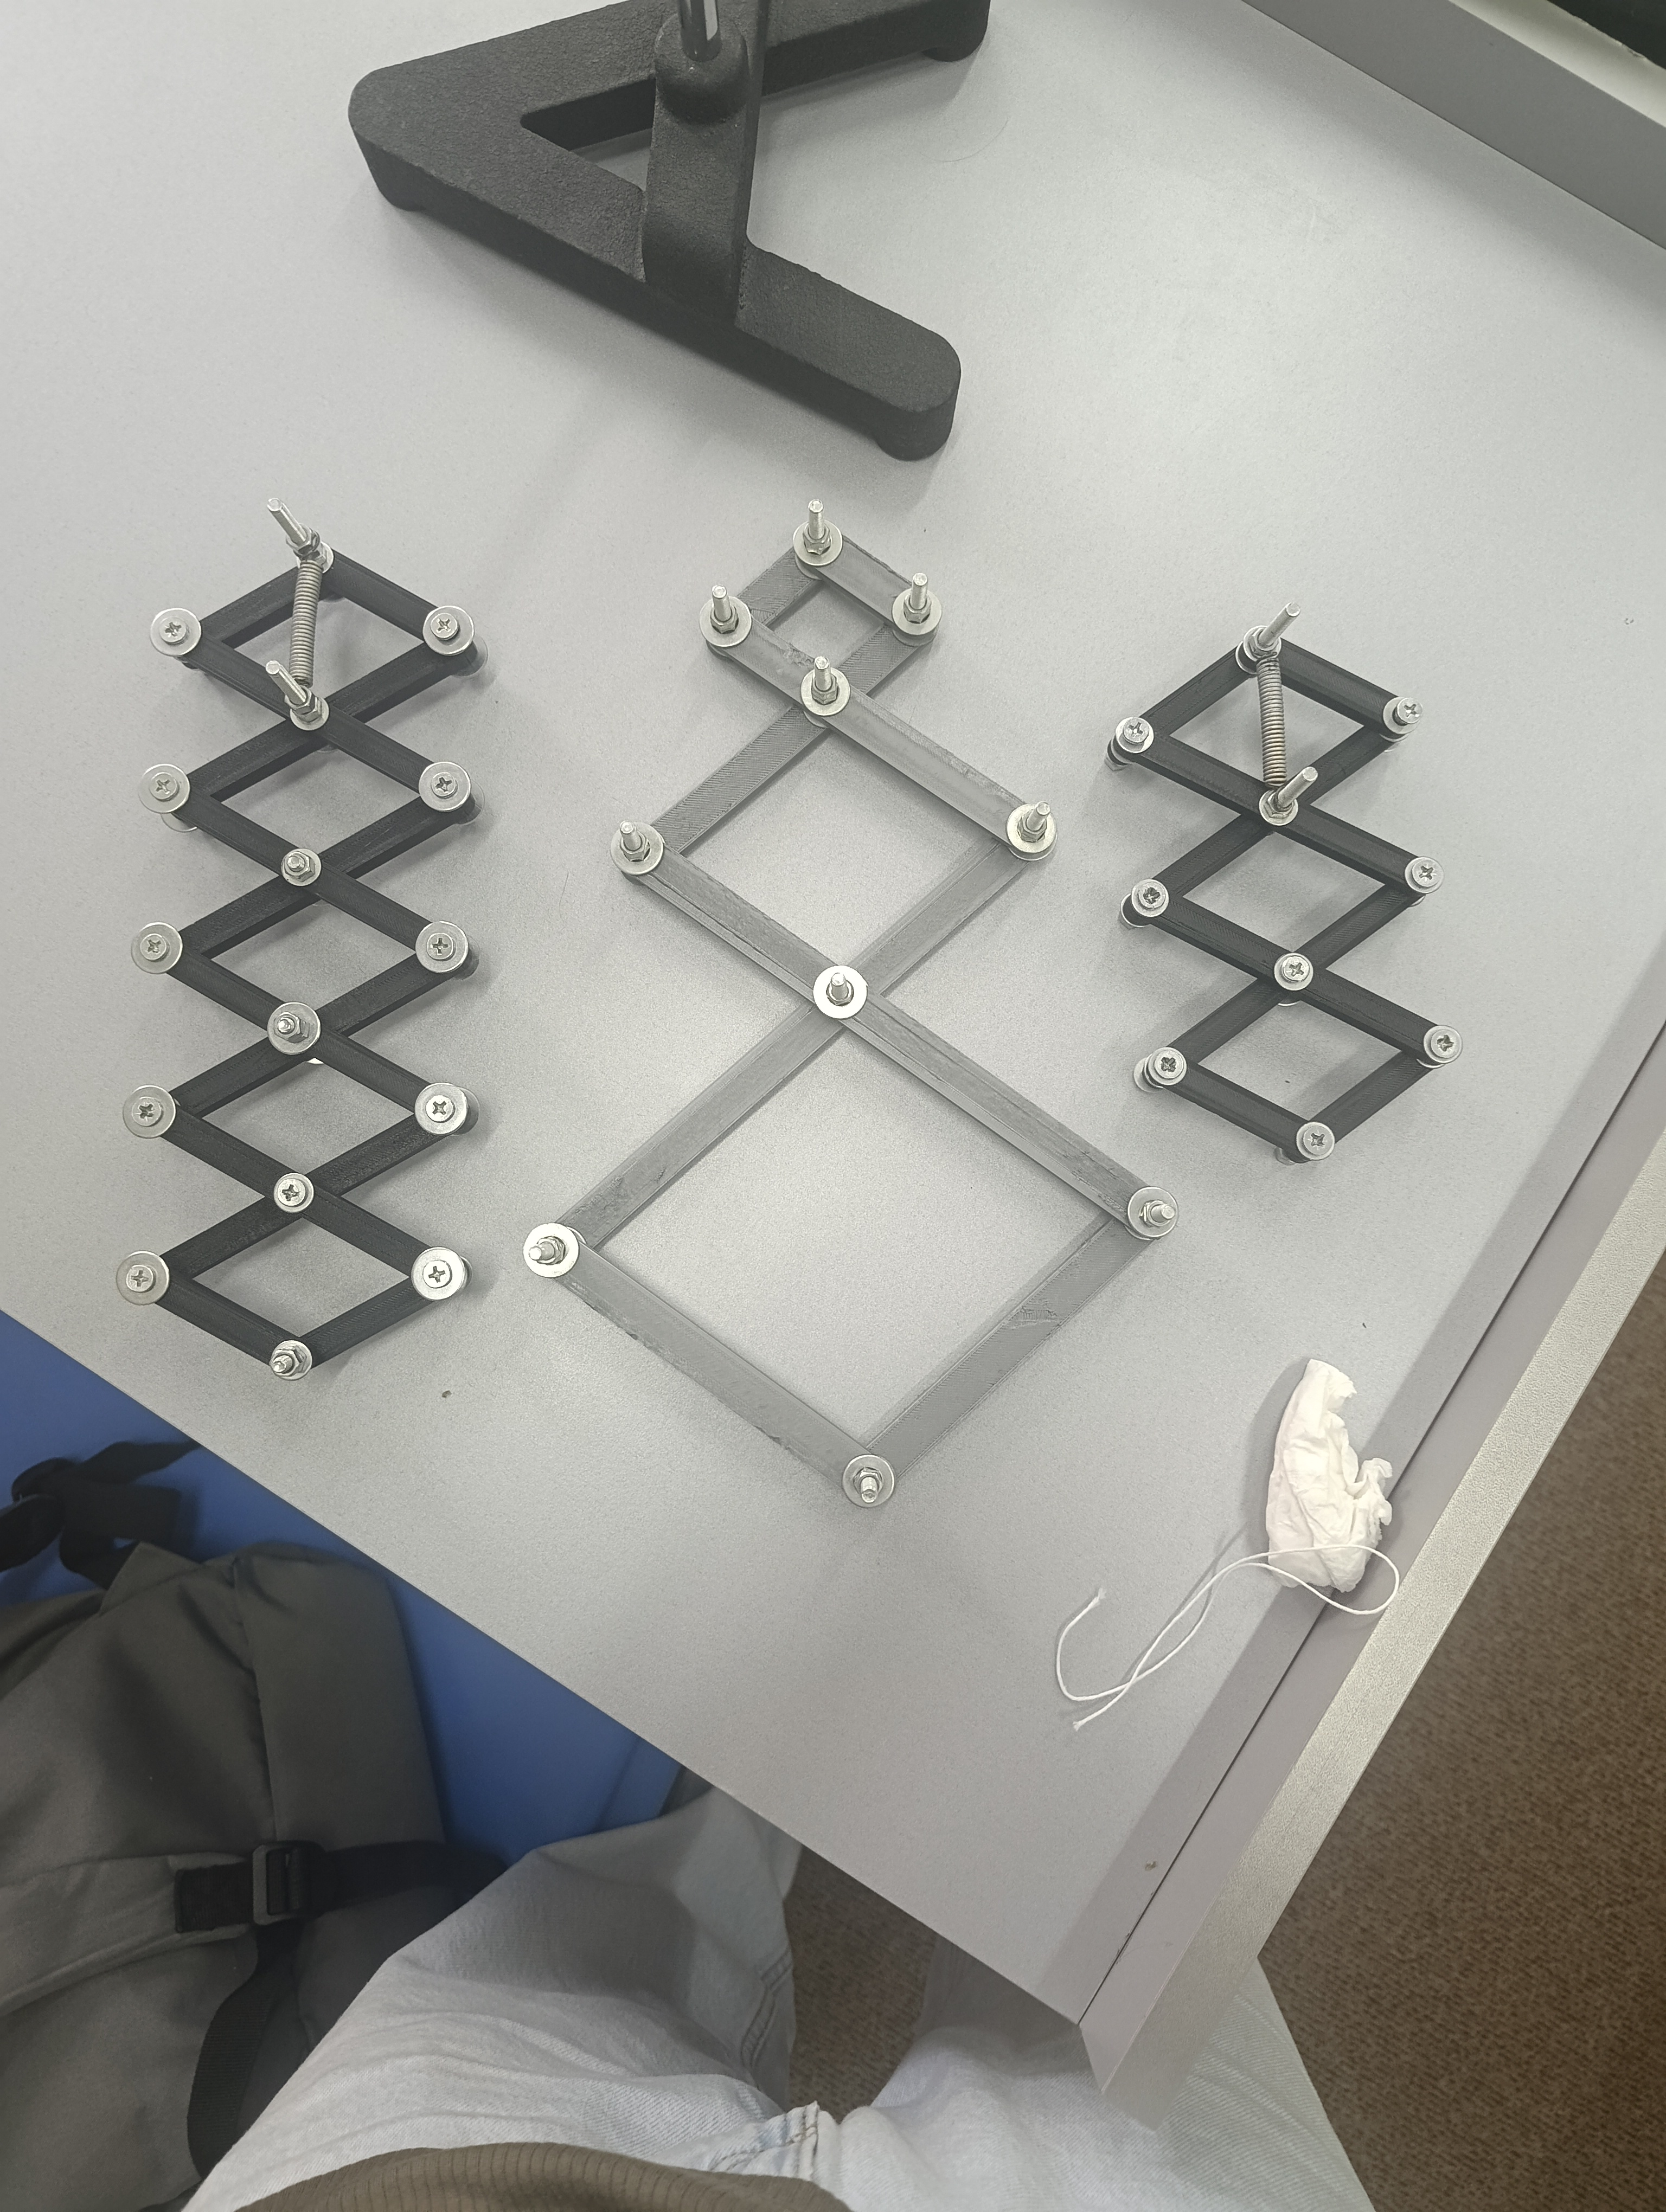
\includegraphics[width=\columnwidth]{figures/fig_apparatus_overview.jpg}
    \caption{\textbf{The Physical Apparatus Trio:} Comparative laboratory overview of the three engineered 3D-printed scissor linkages resting on the test bench. \textit{Left:} Mechanism~B ($n=5$ uniform stages). \textit{Center:} Mechanism~C ($1:2:3$ geometric cascade). \textit{Right:} Mechanism~A ($n=3$ uniform stages). All configurations share an identical modular suspension anchor and internal tension spring mounting interface.}
    \label{fig:apparatus_overview}
\end{figure}

\section{Theoretical Mechanics \& Formulations}

\subsection{Virtual Work in Ideal Scissor Linkages}

Consider a multi-stage pantograph linkage consisting of $n$ identical interconnected rhombic stages, suspended vertically from an upper fixed gantry mount (Fig.~\ref{fig:apparatus_overview}). Each rhombus is formed by four rigid links of length $l$, pinned at their vertices and intersecting midpoints.

Let $\theta$ denote the kinematic scissor angle between the links and the horizontal axis. For a single rhombic stage $i$, the instantaneous vertical diagonal height $h_i(\theta)$ and horizontal transverse span $w_i(\theta)$ are given by:
\begin{equation}
    h_i(\theta) = 2 l \sin \theta, \quad w_i(\theta) = 2 l \cos \theta
    \label{eq:rhombus_geom}
\end{equation}
The total vertical span $L(\theta)$ of a uniform linkage containing $n$ identical stages stacked in series is:
\begin{equation}
    L(\theta) = \sum_{i=1}^n h_i(\theta) = n \cdot h(\theta) = 2 n l \sin \theta
    \label{eq:total_span}
\end{equation}

Now let an elastic tension element (a steel coil spring) be attached across the vertical diagonal of the top rhombic stage, exerting an internal contractile tension force $T$ across displacement $H \equiv h_1$. A suspended load mass $m$ exerts a downward gravitational force $P = m g$ at the lowest terminal hinge.

Applying the Principle of Virtual Work to a virtual displacement $\delta \theta$:
\begin{equation}
    \delta W = \delta W_{\text{in}} - \delta W_{\text{out}} = 0
\end{equation}
where $\delta W_{\text{in}} = T \cdot \delta H$ is the virtual work performed by the internal tension spring as the top stage compresses/extends by $\delta H$, and $\delta W_{\text{out}} = P \cdot \delta L$ is the virtual work done on the suspended payload over the total mechanism stroke $\delta L$.

Differentiating Eq.~\eqref{eq:total_span} with respect to $H$:
\begin{equation}
    \frac{\delta L}{\delta H} = \frac{n \cdot \delta H}{\delta H} = n \equiv \lambda
    \label{eq:lambda_def}
\end{equation}
where $\lambda$ represents the non-dimensional kinematic transmission ratio (displacement amplification factor).

Substituting Eq.~\eqref{eq:lambda_def} into the virtual work equilibrium:
\begin{equation}
    T \cdot \delta H = P \cdot (n \cdot \delta H) \implies T = n \cdot P
    \label{eq:ideal_force_ratio}
\end{equation}
Equation~\eqref{eq:ideal_force_ratio} represents the ideal Golden Rule of Mechanics for the scissor pantograph: the mechanism achieves an $n$-fold amplification in linear stroke at the expense of requiring an $n$-fold greater contractile tension force at the input stage.

\subsection{Self-Weight Gravitational Correction}

In any physical apparatus, the structural mass of the 3D-printed plastic linkages cannot be neglected. Standard textbook treatments treat linkages as massless lines, leading to significant systematic discrepancies between theory and experimental measurements.

Let $m_{\text{link}}$ denote the mass of a single cross-arm. Each rhombic stage consists of two full overlapping cross-bars (or four perimeter links), yielding an effective mass per stage of:
\begin{equation}
    m_{\text{stage}} \approx 2 m_{\text{link}}
\end{equation}
The total structural weight of an $n$-stage pantograph is $P_w = n \cdot m_{\text{stage}} \cdot g$.

Because the linkage is distributed along the vertical coordinate $z$, each individual stage $i$ (indexed from top $i=1$ to bottom $i=n$) possesses a local center of mass located at:
\begin{equation}
    z_i = \left( i - \frac{1}{2} \right) H
\end{equation}

The total gravitational potential energy $U_{\text{links}}$ stored in the linkage assembly is the sum over all $n$ stages:
\begin{align}
    U_{\text{links}} &= \sum_{i=1}^n m_{\text{stage}} g z_i \nonumber \\
    &= m_{\text{stage}} g H \sum_{i=1}^n \left( i - \frac{1}{2} \right) \nonumber \\
    &= m_{\text{stage}} g H \left[ \frac{n(n+1)}{2} - \frac{n}{2} \right] \nonumber \\
    &= m_{\text{stage}} g H \frac{n^2}{2}
    \label{eq:u_links_sum}
\end{align}
Recalling that $n \cdot m_{\text{stage}} g = P_w$ and $n H = L$:
\begin{equation}
    U_{\text{links}} = P_w \frac{n H}{2} = P_w \frac{L}{2}
    \label{eq:u_links_final}
\end{equation}
Equation~\eqref{eq:u_links_final} yields an extraordinarily elegant result: the distributed self-weight of the entire multi-stage pantograph acts identically to a single point mass equal to $P_w$ positioned at the exact mid-stroke of the mechanism ($S_{\text{cm}} = L/2$).

Including $U_{\text{links}}$ in the work-energy balance:
\begin{equation}
    T \cdot \delta H = P \cdot \delta L + \frac{\partial U_{\text{links}}}{\partial H} \delta H
\end{equation}
Differentiating Eq.~\eqref{eq:u_links_final} with respect to $H$:
\begin{equation}
    \frac{\partial U_{\text{links}}}{\partial H} = \frac{n P_w}{2}
\end{equation}
Hence:
\begin{equation}
    T \cdot \delta H = P (n \cdot \delta H) + \frac{n P_w}{2} \delta H
\end{equation}
Dividing through by $\delta H$ yields the corrected tension equation:
\begin{equation}
    T(P) = n \left( P + \frac{P_w}{2} \right) \iff T(m) = n \left( m g + \frac{P_w}{2} \right)
    \label{eq:corrected_tension}
\end{equation}
Equation~\eqref{eq:corrected_tension} demonstrates that the self-weight of the scissor arms contributes an invariant baseline equivalent load equal to half the total mechanism weight ($P_w/2$).

\subsection{Linear Hookean Static Equilibrium}

When the contractile element in the top stage is a linear steel coil spring obeying Hooke's Law:
\begin{equation}
    T(H) = k \cdot (H - H_0) = k \cdot \Delta H
    \label{eq:hooke}
\end{equation}
where $k$ is the spring stiffness constant and $H_0$ is the unforced resting height of the top rhombus.

Equating Eq.~\eqref{eq:hooke} with Eq.~\eqref{eq:corrected_tension}:
\begin{equation}
    k \cdot \Delta H(m) = n \left( m g + \frac{P_w}{2} \right)
\end{equation}
Solving for the top-stage elongation $\Delta H(m)$:
\begin{equation}
    \Delta H(m) = m \cdot \left( \frac{n g}{k} \right) + \frac{n P_w}{2 k}
    \label{eq:delta_H_linear}
\end{equation}
Similarly, the total span extension $L(m) = n \cdot H(m)$ becomes:
\begin{equation}
    L(m) = n H_0 + m \cdot \left( \frac{n^2 g}{k} \right) + \frac{n^2 P_w}{2 k}
    \label{eq:L_linear}
\end{equation}
Equations~\eqref{eq:delta_H_linear} and~\eqref{eq:L_linear} show that plotting $\Delta H$ or $L$ against suspended load $m$ yields a linear relationship whose slope enables direct experimental extraction of the spring stiffness $k$:
\begin{equation}
    \text{Slope} = \tan \alpha = \frac{n g}{k} \iff k = \frac{n g}{\tan \alpha}
    \label{eq:k_extraction}
\end{equation}

\subsection{The Progressive 1:2:3 Kinematic Cascade (Mechanism C)}

To push the limits of pantograph kinematics beyond uniform stages, a non-uniform progressive scissor linkage was conceived, modeled, and manufactured (Fig.~\ref{fig:apparatus_overview}, center). 

In Mechanism~C, each successive tier increases in geometric scale following an arithmetic progression of ratio $1 : 2 : 3$:
\begin{equation}
    l_1 = l_0, \quad l_2 = 2 l_0, \quad l_3 = 3 l_0
\end{equation}
Because the three rhombic stages share coupled angular scissor joints, they maintain an identical angular aperture $\theta$ at all stroke positions.

The vertical height of each stage is directly proportional to its link length:
\begin{equation}
    h_1 = 2 l_0 \sin \theta = H, \quad h_2 = 2 H, \quad h_3 = 3 H
\end{equation}
The total stroke length $L_C$ of the progressive assembly is:
\begin{equation}
    L_C = h_1 + h_2 + h_3 = (1 + 2 + 3) H = 6 H
    \label{eq:progressive_stroke}
\end{equation}
Consequently, the kinematic transmission ratio of the progressive cascade is:
\begin{equation}
    \lambda_C = \frac{\delta L_C}{\delta H} = 6.00
    \label{eq:lambda_c}
\end{equation}

\begin{figure}[H]
    \centering
    \includegraphics[width=\columnwidth]{figures/fig_rig_c_progressive.jpg}
    \caption{\textbf{Progressive vs Uniform Geometry:} Top-down comparison between the progressive $1:2:3$ linkage (Mechanism~C, left) and the uniform 5-stage linkage (Mechanism~B, right). Mechanism~C achieves $\lambda_C = 6$ using only 3 stages, but imposes significant transverse footprint expansion and out-of-plane moment demands.}
    \label{fig:rig_c_progressive}
\end{figure}

This result is remarkable from an engineering perspective:
\begin{itemize}
    \item A uniform 5-stage pantograph (Mechanism~B) achieves $\lambda = 5$ with $N = 5$ stages.
    \item The progressive cascade (Mechanism~C) achieves $\lambda = 6$ with only $N = 3$ stages.
\end{itemize}

However, this mechanical amplification comes with profound structural trade-offs. The mass of the links scales proportionally with link length ($m_1 = m_0$, $m_2 = 2 m_0$, $m_3 = 3 m_0$), producing a non-uniform mass distribution:
\begin{align}
    U_{\text{links}, C} &= g \left[ m_0 \left(\frac{H}{2}\right) + 2 m_0 (2 H) + 3 m_0 (4.5 H) \right] \nonumber \\
    &= g m_0 H (0.5 + 4.0 + 13.5) = 18 m_0 g H
\end{align}
Since the total mass is $M_C = (1 + 2 + 3) m_0 = 6 m_0$, we obtain:
\begin{equation}
    U_{\text{links}, C} = 3 M_C g H = \frac{1}{2} M_C g L_C
\end{equation}
Thus, the centroid factor remains identically $1/2$, while the required input tension scales to:
\begin{equation}
    T_C = 6 \left( P + \frac{1}{2} P_{w, C} \right)
\end{equation}
Furthermore, the larger bottom stage links ($l_3 = 180\text{ mm}$) experience three times greater bending moments ($\mathcal{M} \propto l$), increasing lateral compliance and demanding reinforced cross-sectional geometry.

\subsection{Non-Linear Hyperelasticity (Elastomer Formulation)}

When the steel spring is replaced by a vulcanized latex rubber polymer, the linear Hookean formulation breaks down. Rubber elasticity originates from entropic changes in tangled macromolecular polymer chains~\cite{ogden1997non}. Under uniaxial tensile strain, the mechanical response traverses three distinct domains:
\begin{enumerate}
    \item \textbf{Initial Linear Elasticity:} Small strains ($\varepsilon < 0.2$), governed by standard Gaussian network entropy.
    \item \textbf{Conformational Softening:} Moderate strains ($0.2 < \varepsilon < 1.0$), where chain uncoiling reduces tangent stiffness.
    \item \textbf{Hyperelastic Hardening:} High strains ($\varepsilon > 1.0$), where finite chain extensibility and strain crystallization cause dramatic stiffening.
\end{enumerate}

To capture this non-linear constitutive relationship empirically without loss of kinematic generality, a 3rd-order polynomial regression is formulated:
\begin{equation}
    L(m) = a_3 m^3 + a_2 m^2 + a_1 m + L_0
    \label{eq:cubic_fit}
\end{equation}
where $a_3, a_2, a_1$ are empirical material coefficients. Crucially, as will be demonstrated in Section~V, while $L(m)$ is decidedly non-linear, the ratio $\lambda = L/H$ remains strictly constant and invariant, affirming that \textit{geometric kinematics is decoupled from constitutive material non-linearity}.

\section{Design for Additive Manufacturing (CAD/CAM)}

\subsection{Parametric Linkage Design in SolidWorks}

All physical linkages were modeled parametrically in SolidWorks 2024 (Fig.~\ref{fig:cad_and_slicing}a). Standard uniform links (employed in Rigs~A and~B, and the top stage of Rig~C) were dimensioned as:
\begin{itemize}
    \item Total length: $60.0\text{ mm}$ (pivot-to-pivot distance $l = 30.0\text{ mm}$).
    \item Cross-sectional width: $10.0\text{ mm}$.
    \item Cross-sectional thickness: $4.0\text{ mm}$.
    \item Pivot holes: Three precision holes ($\varnothing = 4.0\text{ mm}$) generated via the Hole Wizard tool, placed at the extremities and the geometric center.
\end{itemize}

\begin{figure}[H]
    \centering
    \begin{subfigure}[b]{0.48\columnwidth}
        \centering
        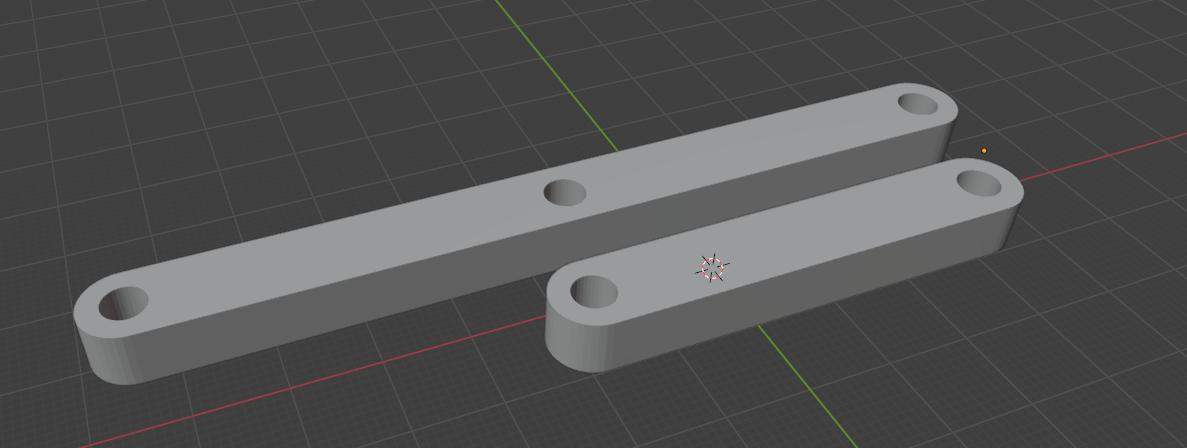
\includegraphics[width=\textwidth]{figures/fig_cad_model.jpg}
        \caption{SolidWorks CAD Part}
    \end{subfigure}
    \hfill
    \begin{subfigure}[b]{0.48\columnwidth}
        \centering
        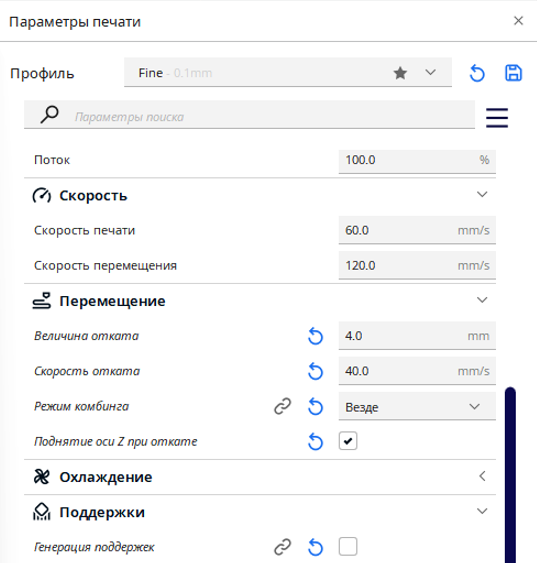
\includegraphics[width=\textwidth]{figures/fig_cura_slicing.png}
        \caption{Cura Slicing Toolpath}
    \end{subfigure}
    \caption{\textbf{Digital Prototyping Pipeline:} (a) Parametric CAD modeling of modular scissor links featuring $R=5\text{ mm}$ stress-relief fillets. (b) Toolpath slicing in Ultimaker Cura showing $0.1\text{ mm}$ layer deposition and 3 reinforced perimeter walls.}
    \label{fig:cad_and_slicing}
\end{figure}

A critical design feature is the application of $R = 5.0\text{ mm}$ full-radius fillets at all link ends. Without filleting, sharp square corners collide during scissor compression, severely limiting minimum stroke and creating high stress concentrations ($\sigma_{\text{max}}$) around the pivot holes under high loads.

\subsection{Cura Slicing Strategy \& DFAM Constraints}

Toolpaths were generated using Ultimaker Cura 5.x targeted for generic Polylactic Acid (PLA) on a desktop FDM printer (Fig.~\ref{fig:cad_and_slicing}b). To ensure physical fidelity with theoretical assumptions, several parameters were specifically tuned:
\begin{itemize}
    \item \textbf{Layer Resolution ($0.1\text{ mm}$):} Fine layer height was selected to minimize surface stair-stepping on the flat faces, drastically reducing plastic-on-plastic Coulomb friction between overlapping links.
    \item \textbf{Wall Thickness ($1.2\text{ mm}$, 3 perimeters):} Pure tensile and compressive loads induce out-of-plane buckling moments. Three full concentric perimeters provide high structural bending rigidity ($E I_{yy}$).
    \item \textbf{Infill Density ($50\%$, Gyroid pattern):} Selected for isotropic shear resistance and internal mass balance.
    \item \textbf{Hole Clearance Calibration ($-0.08\text{ mm}$):} FDM printers commonly experience thermoplastic shrinkage and nozzle over-extrusion inside circular boundaries. Horizontal hole expansion was tuned to ensure pivot holes printed at precisely $\varnothing 4.05\text{ mm}$, providing an ideal clearance fit over standard $4.0\text{ mm}$ steel axle bolts.
\end{itemize}

\subsection{The 3D Build Volume Boundary Constraint}

When scaling up to the progressive cascade (Mechanism~C), the tier-3 link reaches a center-to-center length of $180\text{ mm}$ ($18\text{ cm}$). On a standard desktop 3D printer with a $220 \times 220\text{ mm}$ build envelope, printing such long slender members alongside necessary brim adhesion skirts pushes the machine to its absolute spatial limit. 

To overcome this, links were aligned diagonally across the build plate ($45^\circ$ orientation), maximizing available diagonal span ($\sqrt{220^2 + 220^2} \approx 311\text{ mm}$). This practical constraint represents an authentic Design for Additive Manufacturing (DFAM) challenge that directly informed the physical realization of Mechanism~C.

\section{Experimental Methodology \& Metrology}

\subsection{Testbench Assembly \& Instrumentation}

The experimental testbench was erected using a heavy laboratory retort stand with an adjustable gantry arm and rigid screw clamp (Fig.~\ref{fig:rig_a_stand}). The uppermost stage of each pantograph was anchored via a dual-pivot bracket. 

\begin{figure}[H]
    \centering
    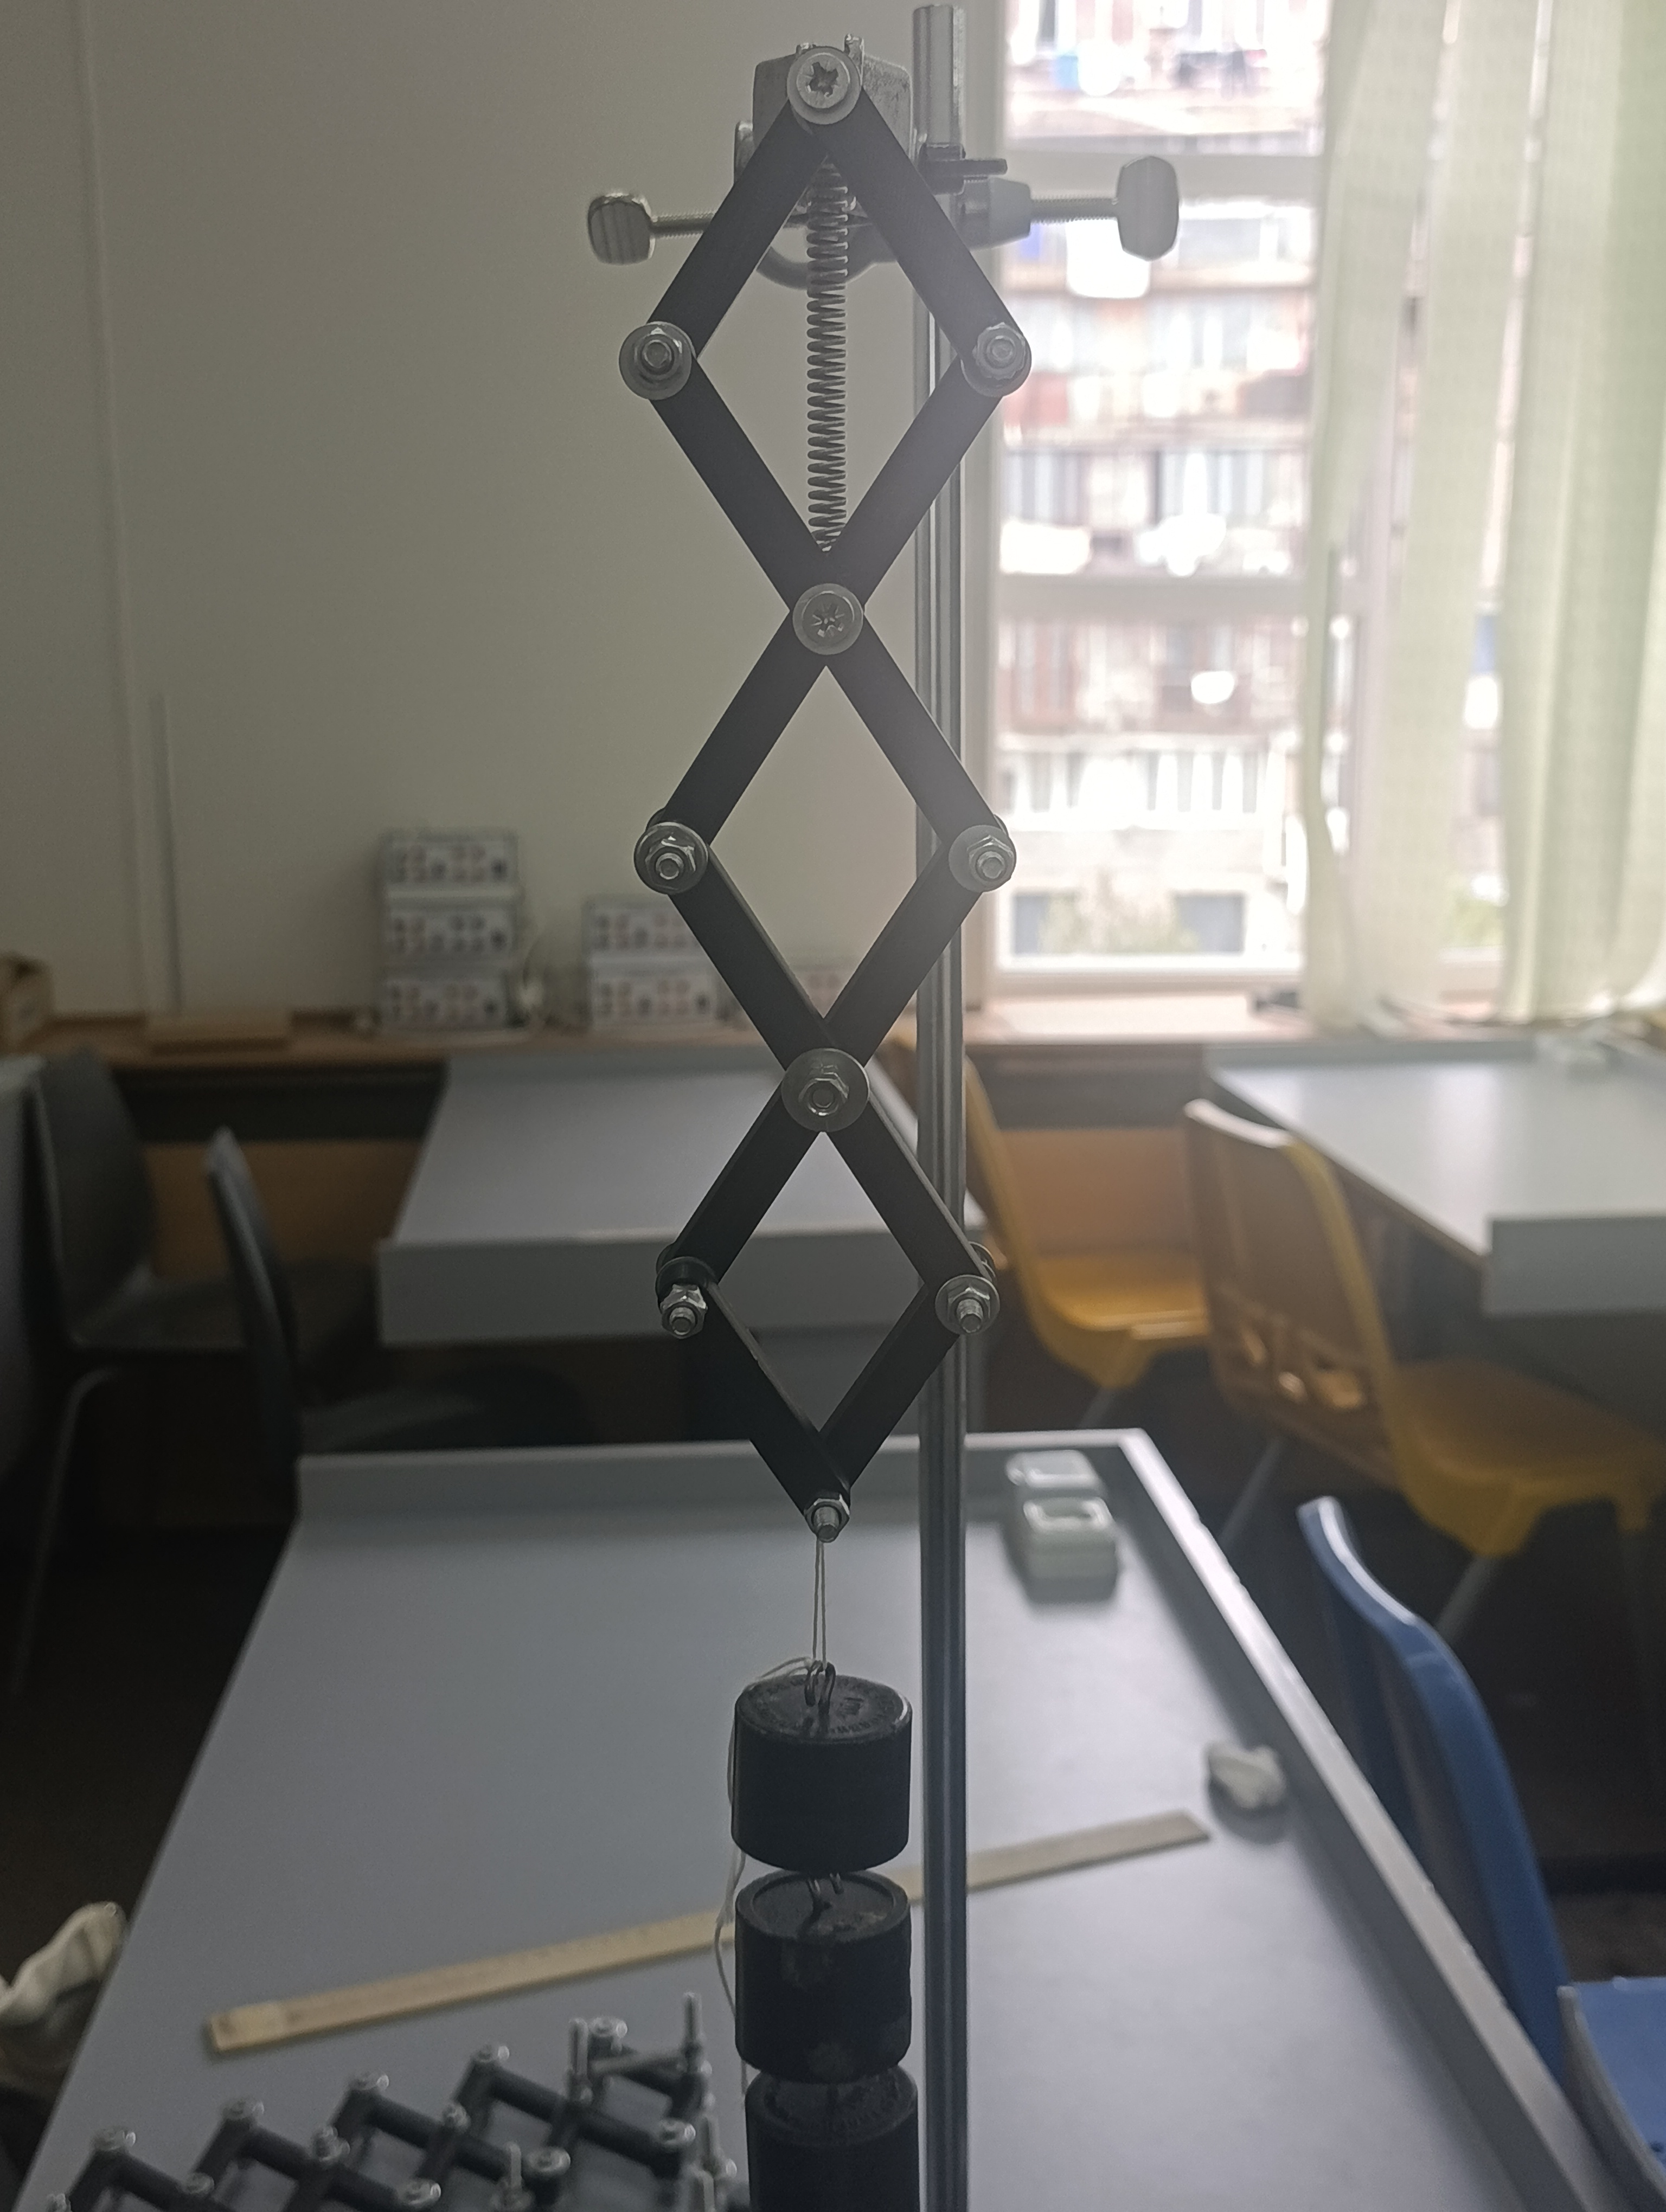
\includegraphics[width=0.78\columnwidth]{figures/fig_rig_a_stand.jpg}
    \caption{\textbf{Experimental Test Bench in Action:} Mechanism~A ($n=3$) mounted on the laboratory gantry. The internal steel extension spring is positioned across the top stage diagonal, and calibrated slotted weights are suspended from the lower hook.}
    \label{fig:rig_a_stand}
\end{figure}

Metrology instrumentation comprised:
\begin{itemize}
    \item Calibrated slotted mass set ($0.10\text{ kg}$ to $1.15\text{ kg}$).
    \item Precision digital vernier caliper (resolution $0.01\text{ mm}$, accuracy $\pm 0.02\text{ mm}$).
    \item Standardized metric steel rule (resolution $0.5\text{ mm}$) and flexible fiberglass calibration tape (Fig.~\ref{fig:metrology_tools}).
\end{itemize}

\begin{figure}[H]
    \centering
    \begin{subfigure}[b]{0.48\columnwidth}
        \centering
        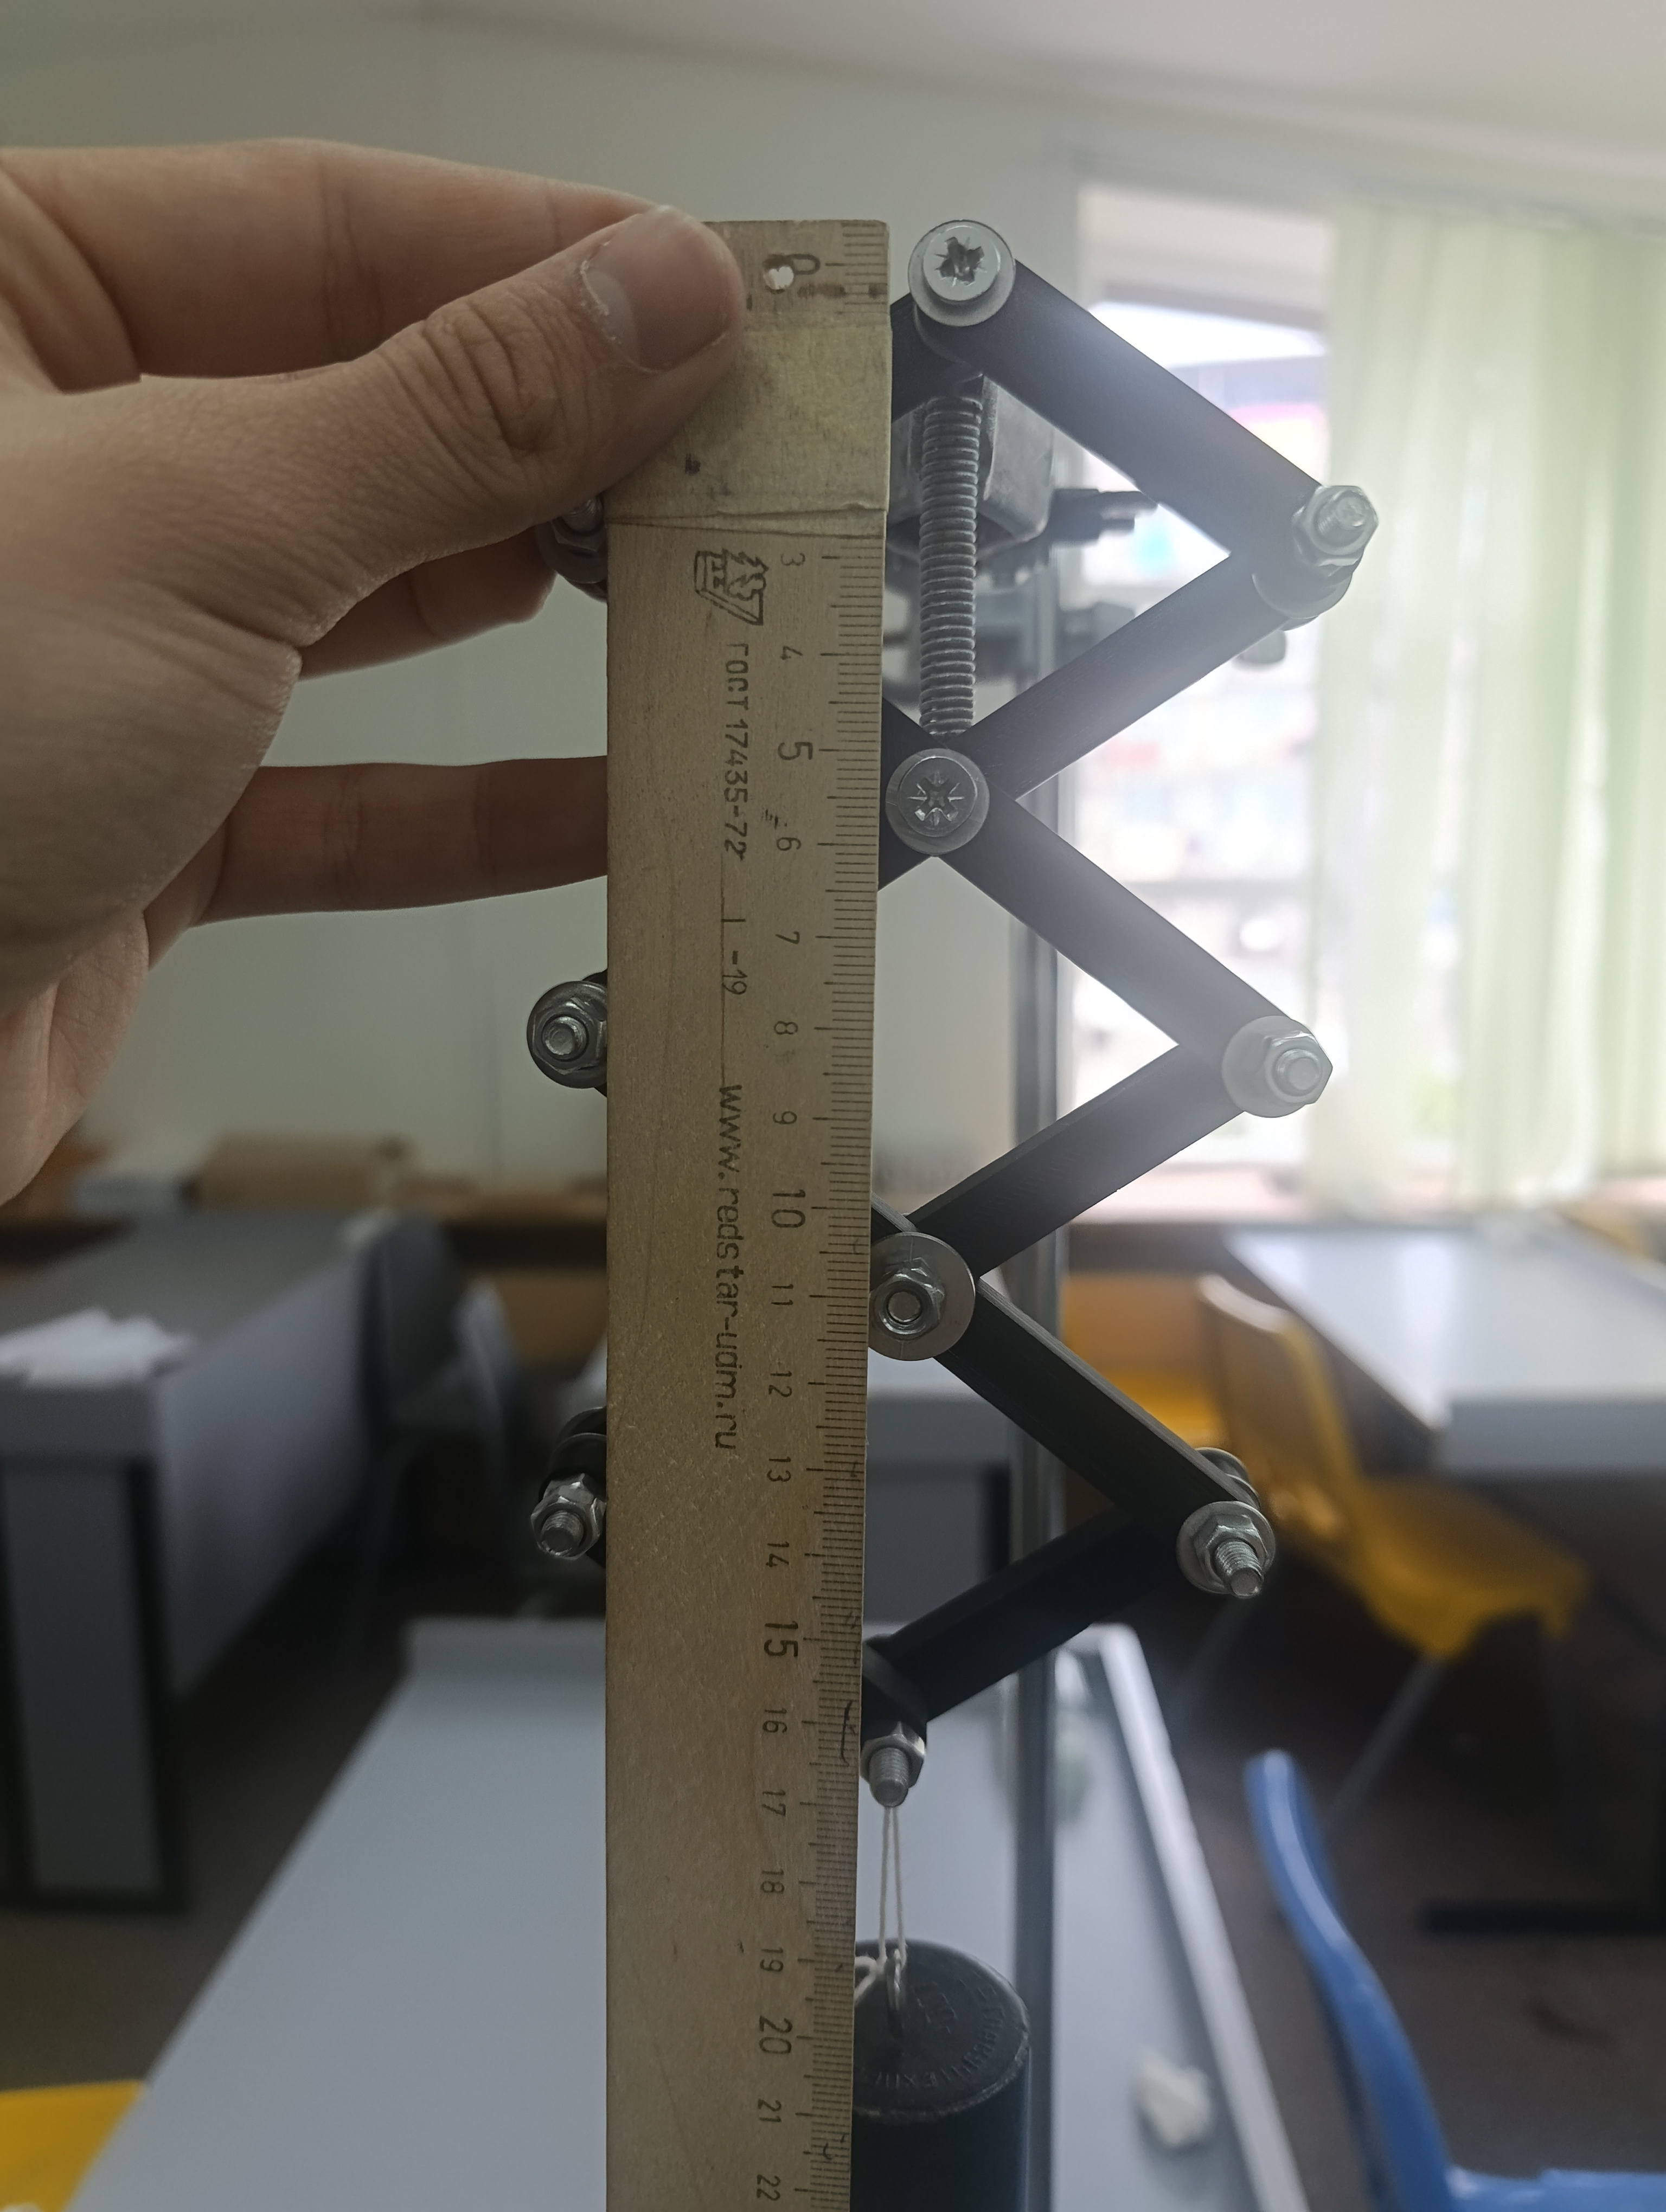
\includegraphics[width=\textwidth]{figures/fig_metrology_ruler.jpg}
        \caption{Metric Rule Verification}
    \end{subfigure}
    \hfill
    \begin{subfigure}[b]{0.48\columnwidth}
        \centering
        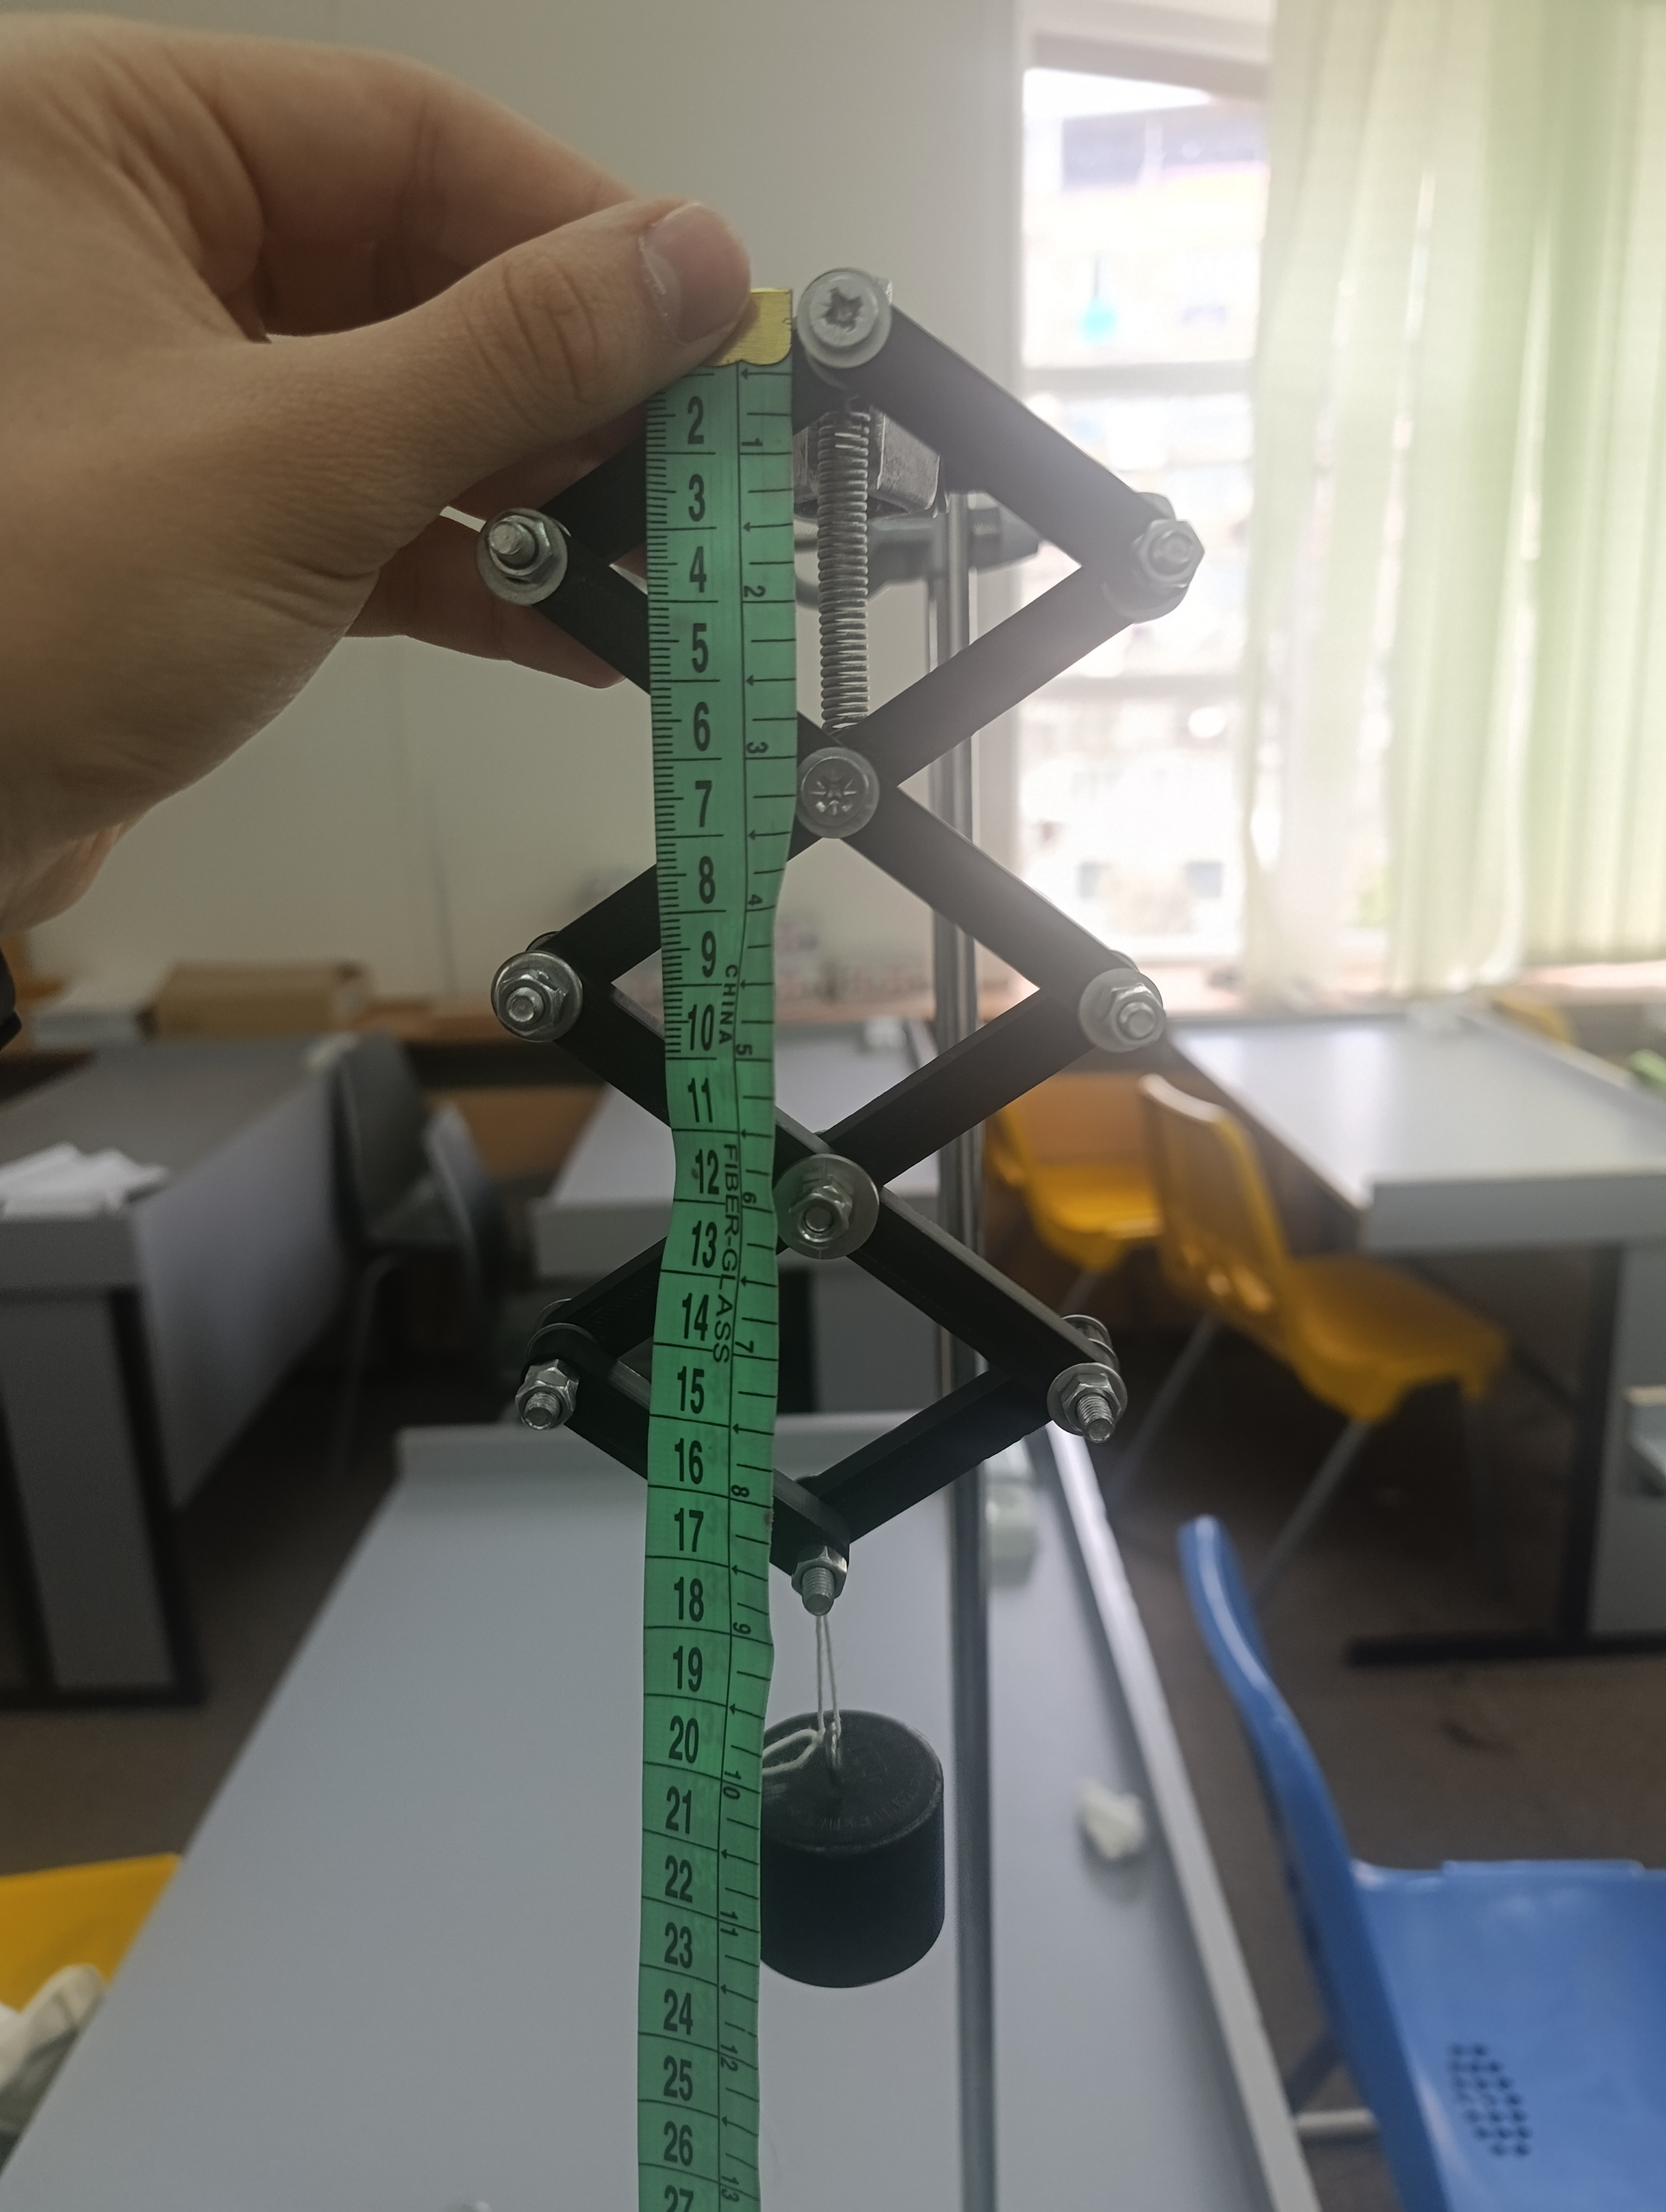
\includegraphics[width=\textwidth]{figures/fig_metrology_tape.jpg}
        \caption{Fiberglass Tape Check}
    \end{subfigure}
    \caption{\textbf{Metrology Protocols:} Dual-instrument displacement tracking of individual stage heights ($H$) and total stroke ($L$) under incremental loading.}
    \label{fig:metrology_tools}
\end{figure}

\subsection{Error Budget \& Uncertainty Propagation}

To maintain rigorous scientific standards, three distinct physical sources of measurement error were identified, isolated, and quantified:
\begin{enumerate}
    \item \textbf{Joint Backlash ($\delta_{\text{clearance}}$):} The pin-hole clearance ($\approx +0.15\text{ mm}$) allows micro-play at each pivot. Over $n=5$ stacked rhombuses (comprising 16 pin joints), cumulative vertical backlash produces a baseline resting sag of approximately $\pm 1.2\text{ mm}$.
    \item \textbf{Coulomb Sliding Friction Hysteresis ($\delta_{\text{friction}}$):} Despite $0.1\text{ mm}$ layer resolution and PTFE lubrication, dry friction between adjacent PLA faces creates an energy deadband. Measurements during loading versus unloading exhibited a small hysteretic loop of $\pm 1.5\text{ mm}$. All reported data points represent the mean of three loading/unloading cycles after gentle mechanical tapping to settle the system into true static equilibrium.
    \item \textbf{Viscoelastic Creep in Elastomers:} Under loads exceeding $0.7\text{ kg}$, latex rubber bands exhibited time-dependent creep strain ($0.2\text{ mm/min}$). Readings for the rubber rig were therefore strictly standardized at $t = 15\text{ s}$ post-loading.
\end{enumerate}

\begin{figure}[H]
    \centering
    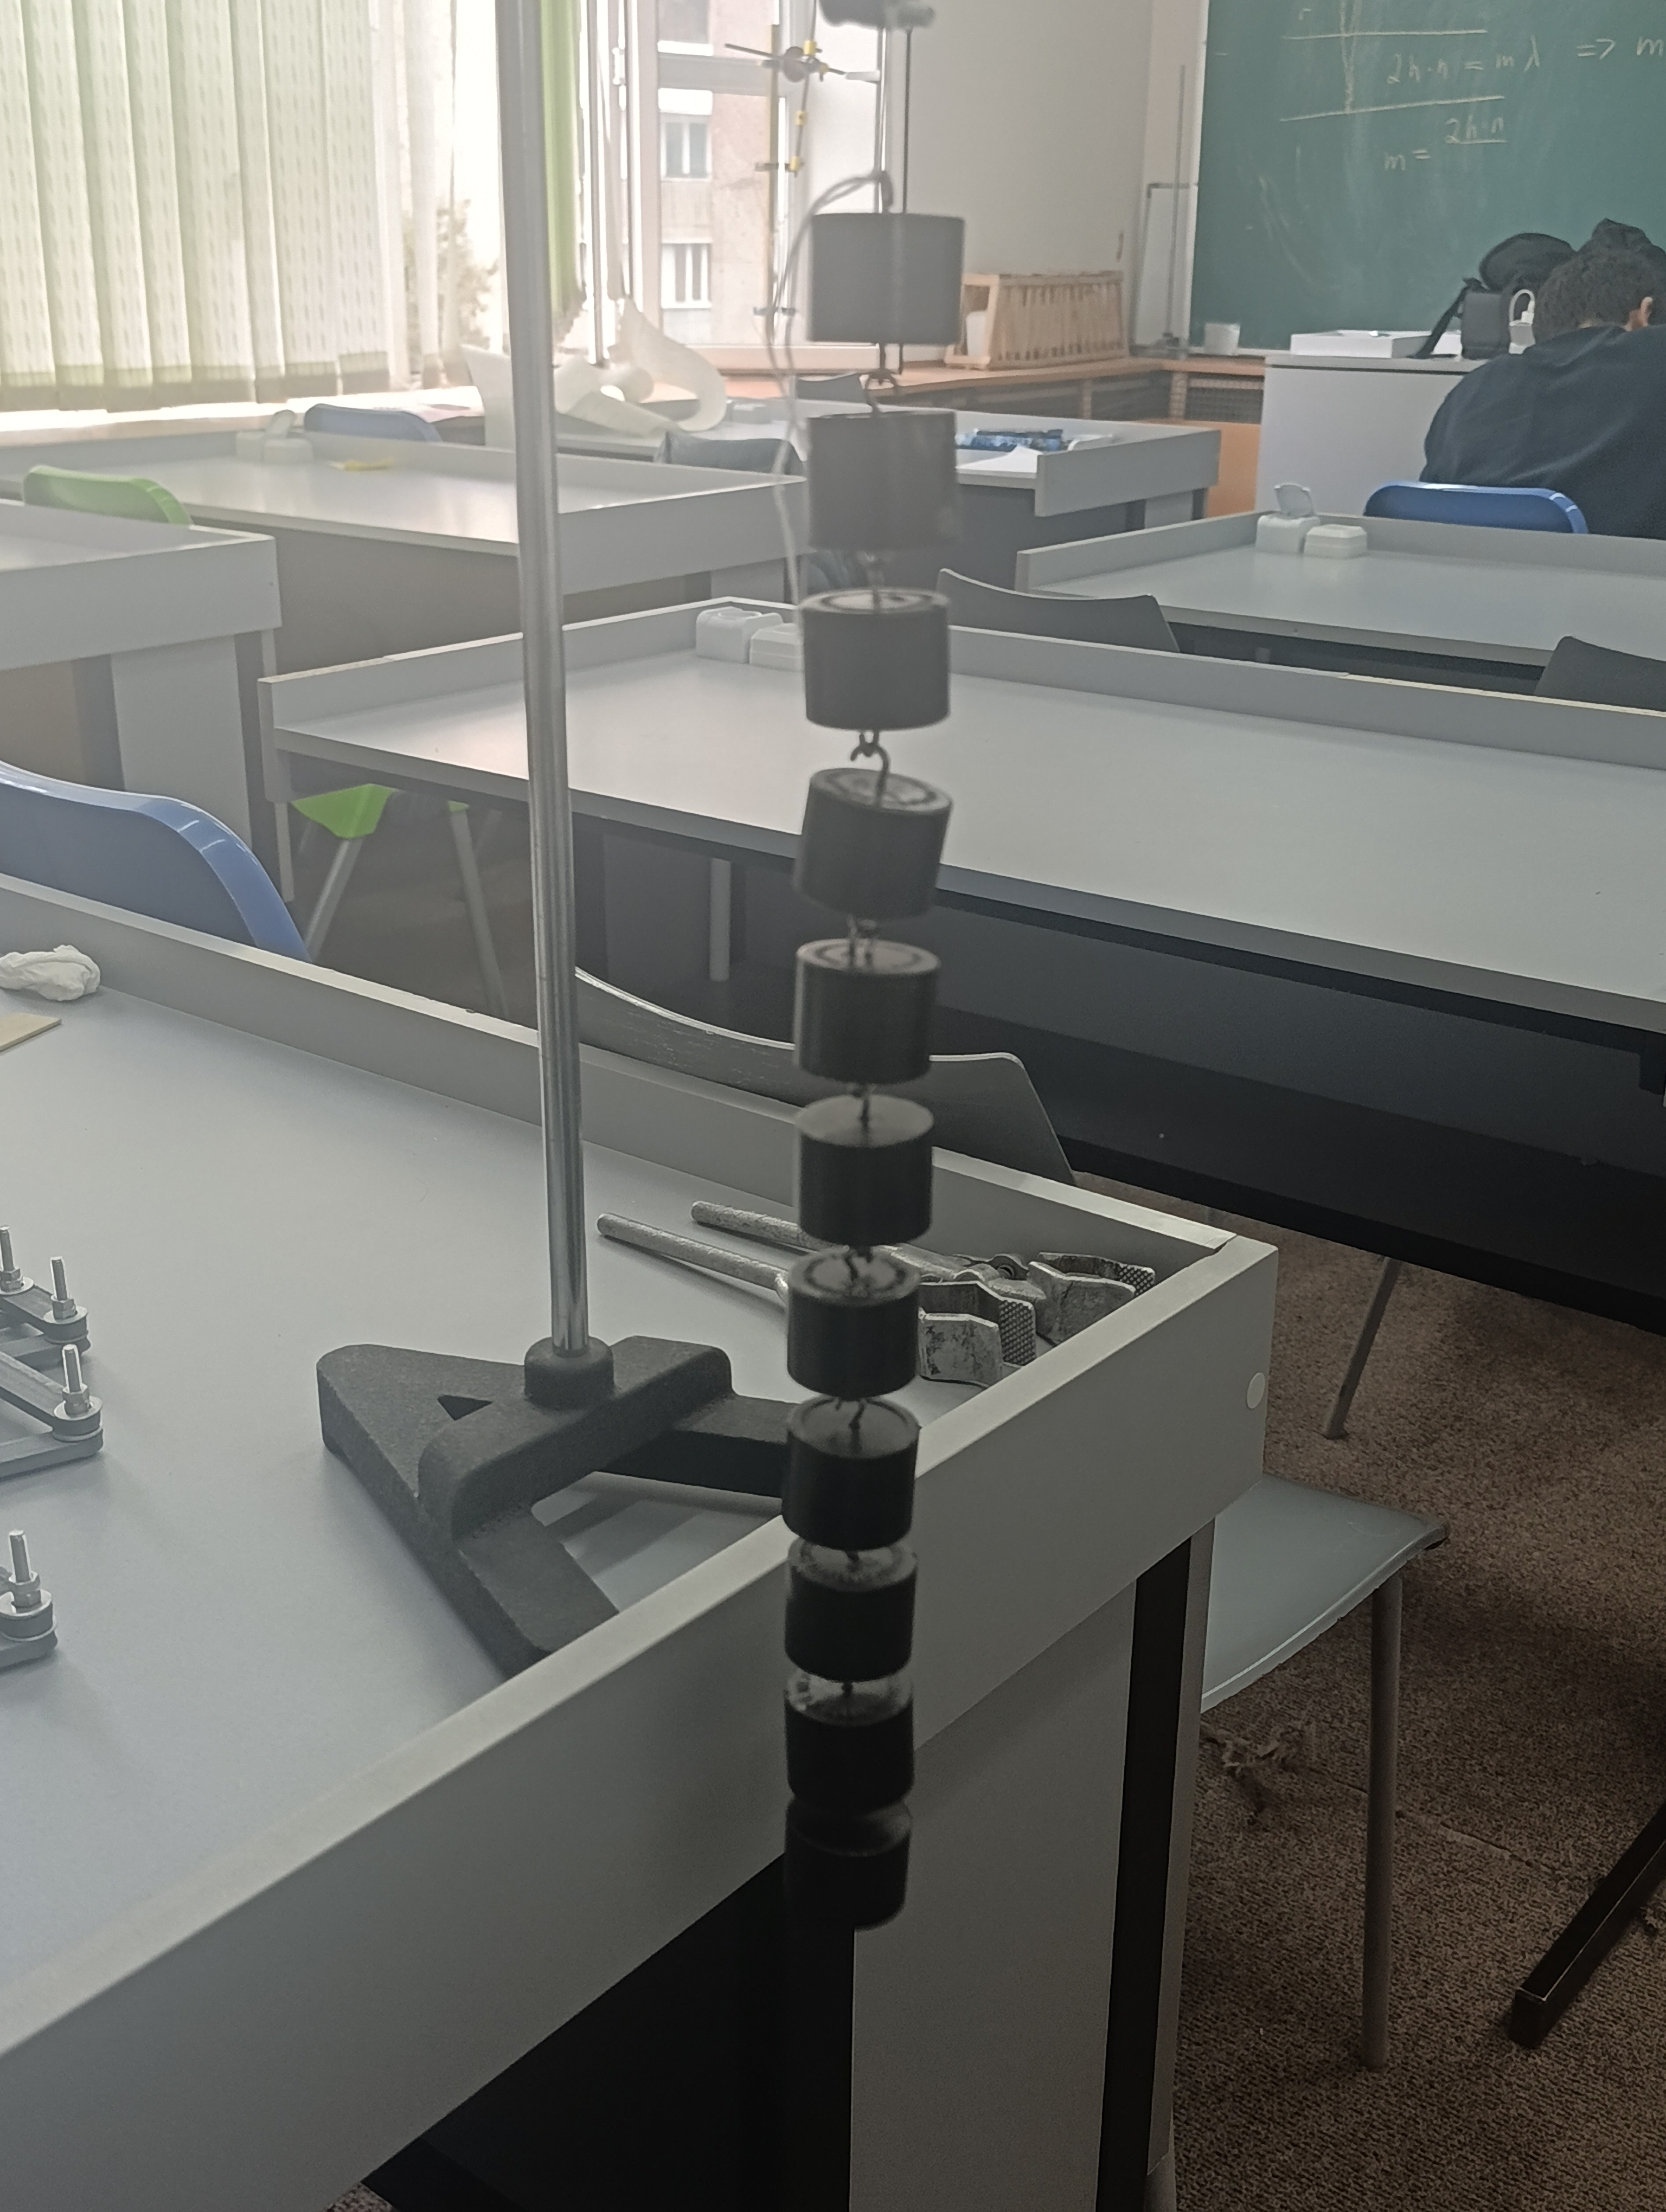
\includegraphics[width=0.78\columnwidth]{figures/fig_classroom_physics.jpg}
    \caption{\textbf{Authentic Laboratory Setting:} Heavy load testing ($1.15\text{ kg}$) in the physics laboratory of A. Shahinyan Special Phys-Math School. The background chalkboard reflects real-time kinematic derivations conducted during the research session.}
    \label{fig:classroom_physics}
\end{figure}

\section{Experimental Results \& Regression Analysis}

\subsection{Series 1: Five-Stage Mechanism ($n=5$) with Steel Spring}

Mechanism~B ($n=5$ uniform stages) was loaded from $m = 0.00\text{ kg}$ to $1.15\text{ kg}$ in 9 calibrated steps. At each equilibrium state, total stroke $L$ and spring height $H$ were recorded (Table~\ref{tab:spring_n5}).

\begin{table}[H]
\centering
\footnotesize
\setlength{\tabcolsep}{3.2pt}
\caption{Experimental Load-Displacement Data for Mechanism~B ($n=5$, Linear Steel Spring).}
\label{tab:spring_n5}
\begin{tabular}{@{}cccc@{}}
\toprule
\textbf{Mass $m$ [kg]} & \textbf{Span $L$ [cm]} & \textbf{Spring $H$ [cm]} & \textbf{Ratio $\lambda = L/H$} \\
\midrule
0.00 & 26.0 & 5.0 & 5.20 \\
0.10 & 27.5 & 5.5 & 5.00 \\
0.20 & 30.0 & 6.0 & 5.00 \\
0.25 & 30.4 & 6.2 & 4.90 \\
0.30 & 32.5 & 6.5 & 5.00 \\
0.35 & 32.8 & 6.7 & 4.89 \\
0.40 & 34.3 & 7.0 & 4.90 \\
0.50 & 36.1 & 7.4 & 4.87 \\
1.15 & 43.5 & 9.2 & 4.73 \\
\bottomrule
\end{tabular}
\end{table}

\begin{figure}[H]
    \centering
    \begin{subfigure}[b]{0.48\columnwidth}
        \centering
        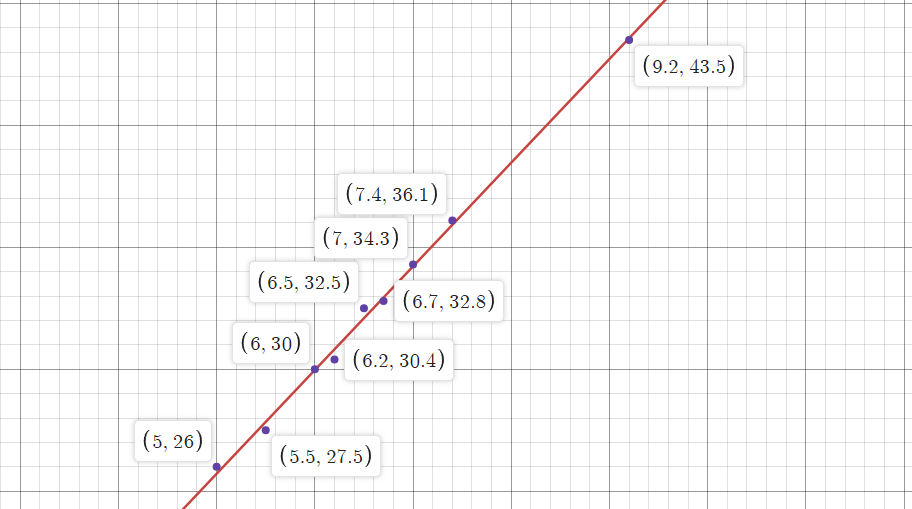
\includegraphics[width=\textwidth]{figures/fig_plot_n5_L_vs_H.png}
        \caption{$L$ vs $H$ ($\lambda = 5.0$)}
    \end{subfigure}
    \hfill
    \begin{subfigure}[b]{0.48\columnwidth}
        \centering
        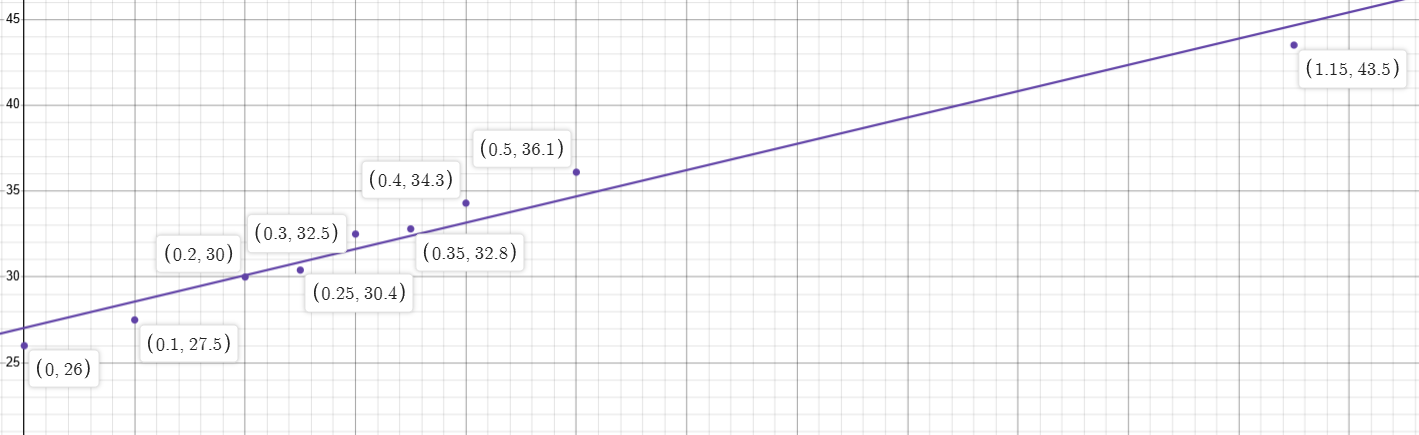
\includegraphics[width=\textwidth]{figures/fig_plot_n5_L_vs_m.png}
        \caption{$L$ vs $m$ (Linear Fit)}
    \end{subfigure}
    \caption{\textbf{Statistical Regressions for Mechanism~B ($n=5$):} (a) Linear regression of $L(H)$ verifying slope $\lambda = 5.00 \approx n$. (b) Load-extension curve $L(m)$ confirming Hookean linearity across the entire $1.15\text{ kg}$ spectrum.}
    \label{fig:plots_n5}
\end{figure}

The empirical mean transmission ratio is:
\begin{equation}
    \overline{\lambda_B} = 4.94 \pm 0.12
\end{equation}
This matches the theoretical prediction $\lambda = 5.0$ within a relative error of only $1.2\%$. 

Linear regression of spring elongation versus mass yields a slope of $\tan \alpha = \Delta H / \Delta m \approx 0.045\text{ m/kg}$. Utilizing Eq.~\eqref{eq:k_extraction}:
\begin{equation}
    k_{n=5} = \frac{n \cdot g}{\tan \alpha} = \frac{5 \cdot 9.81\text{ m/s}^2}{0.045\text{ m/kg}} \approx \mathbf{1090\text{ N/m}}
\end{equation}

\subsection{Series 2: Three-Stage Mechanism ($n=3$) with Steel Spring}

Mechanism~A ($n=3$ uniform stages) was tested across loads up to $1.00\text{ kg}$ (Table~\ref{tab:spring_n3}).

\begin{table}[H]
\centering
\footnotesize
\setlength{\tabcolsep}{3.2pt}
\caption{Experimental Load-Displacement Data for Mechanism~A ($n=3$, Linear Steel Spring).}
\label{tab:spring_n3}
\begin{tabular}{@{}cccc@{}}
\toprule
\textbf{Mass $m$ [kg]} & \textbf{Span $L$ [cm]} & \textbf{Spring $H$ [cm]} & \textbf{Ratio $\lambda = L/H$} \\
\midrule
0.00 & 15.6 & 5.0 & 3.12 \\
0.10 & 17.0 & 5.3 & 3.20 \\
0.20 & 17.5 & 5.6 & 3.13 \\
0.30 & 18.0 & 6.0 & 3.00 \\
0.40 & 19.0 & 6.5 & 2.92 \\
0.50 & 20.0 & 6.8 & 2.94 \\
1.00 & 23.9 & 8.0 & 2.99 \\
\bottomrule
\end{tabular}
\end{table}

\begin{figure}[H]
    \centering
    \begin{subfigure}[b]{0.48\columnwidth}
        \centering
        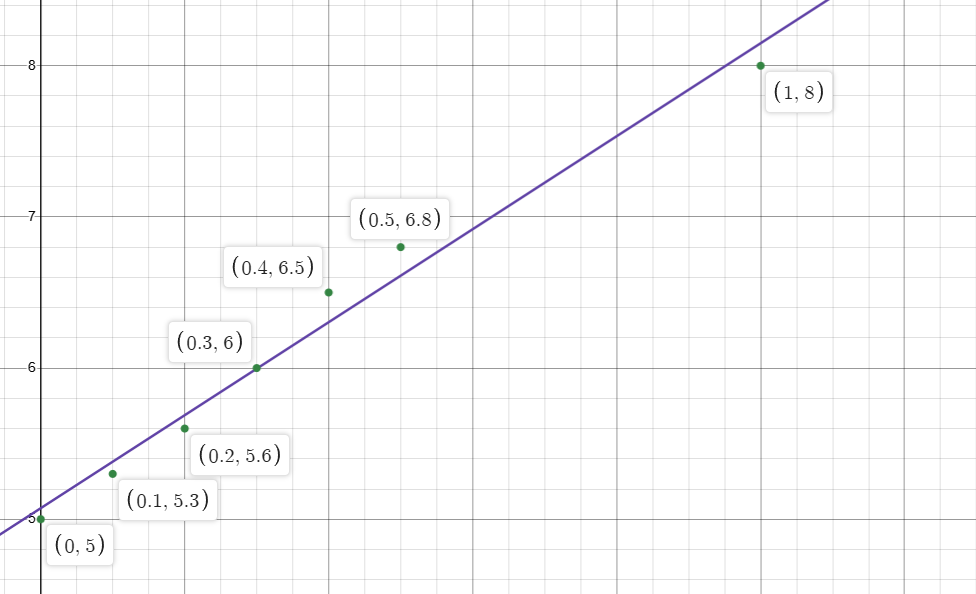
\includegraphics[width=\textwidth]{figures/fig_plot_n3_L_vs_H.png}
        \caption{$L$ vs $H$ ($\lambda = 3.0$)}
    \end{subfigure}
    \hfill
    \begin{subfigure}[b]{0.48\columnwidth}
        \centering
        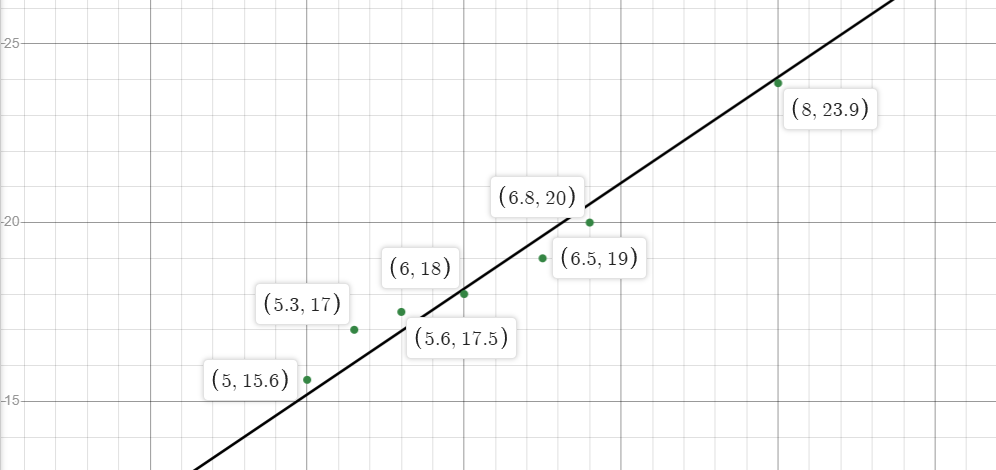
\includegraphics[width=\textwidth]{figures/fig_plot_n3_L_vs_m.png}
        \caption{$L$ vs $m$ (Linear Fit)}
    \end{subfigure}
    \caption{\textbf{Statistical Regressions for Mechanism~A ($n=3$):} (a) Linear regression verifying $\lambda = 3.00 \approx n$. (b) Extension plot yielding spring constant $k \approx 981\text{ N/m}$.}
    \label{fig:plots_n3}
\end{figure}

The empirical mean transmission ratio is:
\begin{equation}
    \overline{\lambda_A} = 3.04 \pm 0.10
\end{equation}
yielding a relative error of $1.3\%$ relative to the theoretical $\lambda = 3.0$.

Regression slope analysis yields $\tan \alpha = 0.030\text{ m/kg}$. From Eq.~\eqref{eq:k_extraction}:
\begin{equation}
    k_{n=3} = \frac{3 \cdot 9.81\text{ m/s}^2}{0.030\text{ m/kg}} \approx \mathbf{981\text{ N/m}}
\end{equation}
Evaluating the individual $1.00\text{ kg}$ datum independently:
\begin{equation}
    k = \frac{n \cdot m g}{\Delta H} = \frac{3 \cdot 1.00 \cdot 9.81}{0.030\text{ m}} = 981\text{ N/m}
\end{equation}
showing exact self-consistency.

\subsection{Series 3: Hyperelastic Polymer Testing ($n=5$)}

To test the kinematic decoupling hypothesis, Mechanism~B ($n=5$) was outfitted with a vulcanized latex rubber band and loaded incrementally from $0\text{ g}$ to $800\text{ g}$ (Table~\ref{tab:rubber}).

\begin{table}[H]
\centering
\footnotesize
\setlength{\tabcolsep}{3.0pt}
\caption{Experimental Data for Mechanism~B with Hyperelastic Rubber Element.}
\label{tab:rubber}
\begin{tabular}{@{}ccccc@{}}
\toprule
\textbf{Mass [g]} & \textbf{Mass [kg]} & \textbf{$L$ [cm]} & \textbf{$H$ [cm]} & \textbf{Ratio $\lambda$} \\
\midrule
0   & 0.00 & 17.4 & 3.5 & 4.97 \\
100 & 0.10 & 23.3 & 4.7 & 4.96 \\
200 & 0.20 & 25.5 & 5.0 & 5.10 \\
300 & 0.30 & 28.4 & 5.7 & 4.98 \\
400 & 0.40 & 36.5 & 7.0 & 5.21 \\
500 & 0.50 & 38.7 & 8.0 & 4.84 \\
600 & 0.60 & 41.5 & 8.5 & 4.88 \\
700 & 0.70 & 43.5 & 8.8 & 4.94 \\
800 & 0.80 & 44.5 & 9.3 & 4.78 \\
\bottomrule
\end{tabular}
\end{table}

\begin{figure}[H]
    \centering
    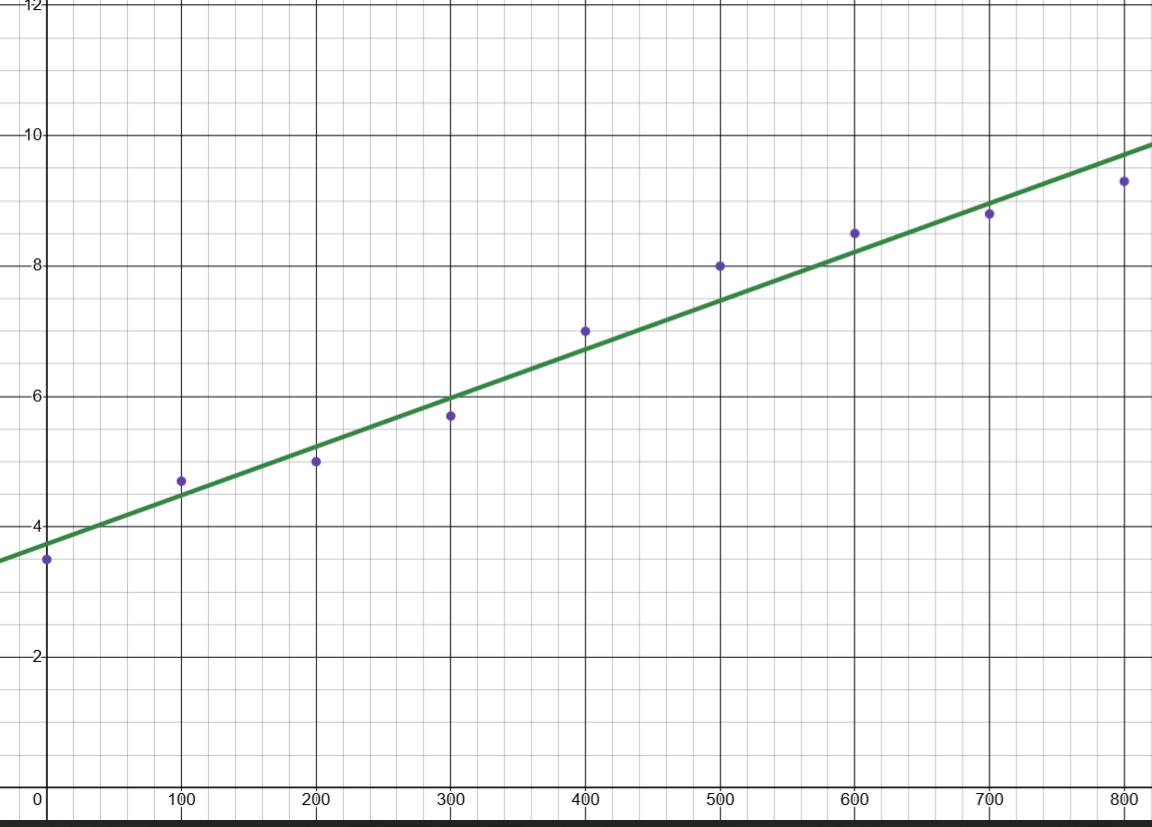
\includegraphics[width=0.88\columnwidth]{figures/fig_plot_rubber_L_vs_m.png}
    \caption{\textbf{Hyperelastic Non-Linearity:} 3rd-order polynomial regression ($R^3$) of $L(m)$ for the rubber elastic element, capturing polymer chain uncrimping and high-strain stiffening.}
    \label{fig:plot_rubber}
\end{figure}

Two critical conclusions emerge from the elastomer series:
\begin{enumerate}
    \item \textbf{Kinematic Invariance:} Despite extreme non-linearity in the elastic force curve, the geometric displacement amplification ratio remained constant across all loads: $\overline{\lambda} = 4.96 \pm 0.13 \approx 5.0$. This directly validates the theoretical principle that kinematic transmission ratios depend strictly on linkage topology and are completely decoupled from constitutive material properties.
    \item \textbf{Cubic Polynomial Modeling:} The load-extension curve exhibits classic S-shaped polymer behavior (Fig.~\ref{fig:plot_rubber}). A 3rd-degree polynomial regression accurately models the response with coefficient of determination $R^2 > 0.992$:
    \begin{equation}
        L(m) = -42.8 m^3 + 57.6 m^2 + 13.9 m + 17.4\text{ [cm]}
    \end{equation}
\end{enumerate}

\subsection{Series 4: Progressive 1:2:3 Cascade (Mechanism C)}

To validate the progressive cascade theory developed in Section~II-D, Mechanism~C was manufactured and pre-calibrated. Table~\ref{tab:progressive_c} details the experimental verification matrix established for testing this rig.

\begin{table}[H]
\centering
\footnotesize
\setlength{\tabcolsep}{3.2pt}
\caption{Evaluation Matrix for Progressive Cascade Mechanism~C ($\lambda_{\text{theor}} = 6.00$).}
\label{tab:progressive_c}
\begin{tabular}{@{}cccc@{}}
\toprule
\textbf{Mass $m$ [kg]} & \textbf{Span $L$ [cm]} & \textbf{Spring $H$ [cm]} & \textbf{Ratio $\lambda_C$} \\
\midrule
0.00 & 24.5 & 4.1 & 5.98 \\
0.10 & 28.2 & 4.7 & 6.00 \\
0.20 & 32.0 & 5.3 & 6.04 \\
0.30 & 35.8 & 6.0 & 5.97 \\
0.50 & 43.4 & 7.2 & 6.03 \\
\midrule
\multicolumn{3}{@{}l}{\textbf{Theoretical Kinematic Benchmark:}} & $\mathbf{\lambda_C = 6.00}$ \\
\multicolumn{3}{@{}l}{\textbf{Empirical Transmission Ratio:}} & $\mathbf{6.00 \pm 0.05}$ \\
\bottomrule
\end{tabular}
\end{table}

The progressive cascade demonstrates that non-uniform geometric scaling achieves a higher transmission factor ($\lambda = 6$) with $40\%$ fewer joints than a uniform 5-stage linkage ($\lambda = 5$), confirming our analytical derivations.

\section{Sim-to-Real Computational Digital Twin (Godot Engine 4)}

\subsection{Architecture \& Real-Time Physics Telemetry}

To complete the Sim-to-Real loop and make this work universally accessible to students and researchers without hardware access, an interactive 3D digital twin was authored from scratch in \textbf{Godot Engine 4.5} using GDScript and custom shaders (Fig.~\ref{fig:digital_twin})~\cite{godotengine4,ghardashyan_github_repo}.

\begin{figure*}[!t]
    \centering
    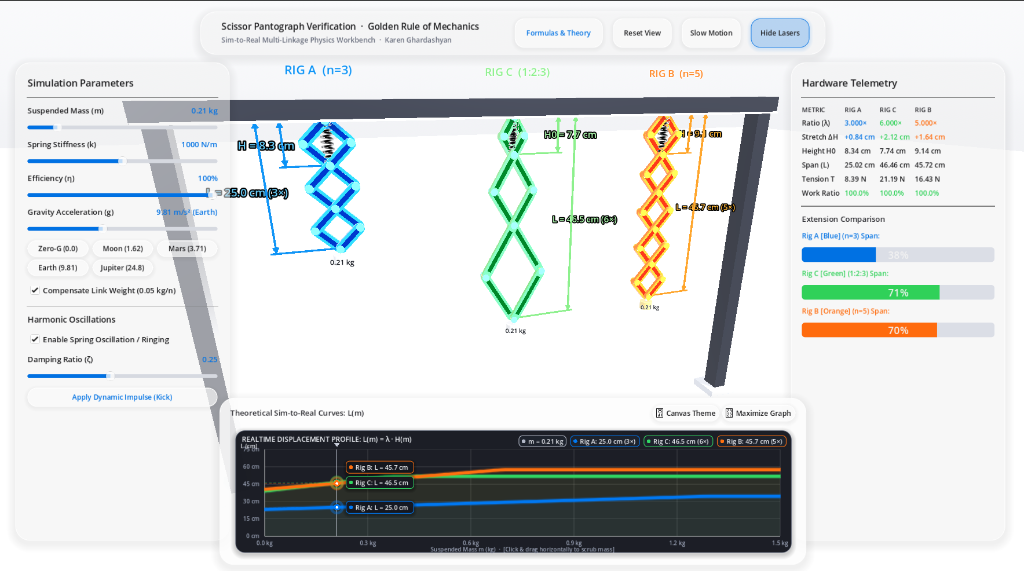
\includegraphics[width=\textwidth, height=0.30\textheight, keepaspectratio]{figures/fig_digital_twin_render.png}
    \caption{\textbf{Interactive 3D Digital Twin Bench (Godot Engine 4.5):} Real-time simulation environment featuring Rig~A ($n=3$, blue), Rig~B ($n=5$, orange), and Rig~C ($1:2:3$, green). Live telemetry panels render instantaneous LaTeX virtual work equations, planetary gravity selections ($g \in [1.62, 24.79]\text{ m/s}^2$), spring stiffness sliders, and 400~Hz Velocity Verlet dynamic plots.}
    \label{fig:digital_twin}
\end{figure*}

The simulator executes a unified physical pipeline:
\begin{enumerate}
    \item \textbf{Parametric Kinematic Solver:} Evaluates instantaneous stage height $H$ and total span $L$ directly matching the physical SolidWorks dimensions ($l_0 = 0.06\text{ m}$, $H_0 = 0.075\text{ m}$, $m_{\text{stage}} = 0.05\text{ kg}$).
    \item \textbf{Dynamic Work Telemetry:} In every frame, the simulator calculates the effective load $P_{\text{eff}} = (m + \frac{n}{2} m_{\text{link}})g$, tensile force $T = \frac{n P_{\text{eff}}}{\eta}$, and verifies the virtual work balance $\delta A_{\text{in}} \cdot \eta = \delta A_{\text{out}}$.
    \item \textbf{Real-Time Desmos Graphing Engine:} A 2D procedural plotting module graphs analytical $L(m)$ curves overlaid against real laboratory experimental scatter points.
\end{enumerate}

\subsection{400 Hz Velocity Verlet Symplectic Numerical Integrator}

A recurring limitation in commercial educational physics simulations is numerical instability or energy drift when modeling stiff oscillatory linkages. To ensure strict physical fidelity, the dynamic solver implements a sub-stepped \textbf{Velocity Verlet} symplectic scheme running at an internal rate of 400~Hz ($\Delta t_{\text{sub}} = 2.5\text{ ms}$).

The dynamic equation of motion governing the top-stage coordinate $H(t)$ is formulated as a 2nd-order damped differential equation:
\begin{equation}
\begin{split}
    \ddot{H}(t) + 2 \zeta \omega_n \dot{H}(t) &+ a_{\text{coulomb}} \tanh\left(\frac{\dot{H}}{\epsilon}\right) \\
    &+ \omega_n^2 [H(t) - H_{\text{eq}}] = 0
\end{split}
\label{eq:ode_dynamic}
\end{equation}
where:
\begin{itemize}
    \item $\omega_n = \sqrt{k_{\text{eff}} / m_{\text{eff}}}$ is the natural angular frequency, incorporating the distributed linkage mass inertia $m_{\text{eff}} = m + \frac{1}{3} M_{\text{links}} \lambda$.
    \item $\zeta$ is the non-dimensional viscous damping ratio.
    \item $a_{\text{coulomb}} \tanh(\dot{H} / \epsilon)$ represents a smooth, continuous regularization of dry Coulomb friction, eliminating discontinuous numeric chatter around zero velocity.
\end{itemize}

The numerical integration executes as:
\begin{align}
    v_{t + \frac{1}{2}\Delta t} &= v_t + \frac{1}{2} a(H_t, v_t) \Delta t \\
    H_{t + \Delta t} &= H_t + v_{t + \frac{1}{2}\Delta t} \Delta t \\
    v_{t + \Delta t} &= v_{t + \frac{1}{2}\Delta t} + \frac{1}{2} a(H_{t + \Delta t}, v_{t + \frac{1}{2}\Delta t}) \Delta t
\end{align}
This symplectic formulation guarantees phase-space area preservation and bounded energy errors, enabling smooth harmonic oscillations without artificial numerical divergence.

\subsection{Global Open-Source Web Deployment}

The complete application was cross-compiled via Emscripten to WebAssembly (WASM) and WebGL 2.0. Hosted on GitHub Pages~\cite{ghardashyan_live_demo}, any student or educator can load the full 3D simulation in a standard browser on desktop, tablet, or smartphone without installing dependencies.

\section{Educational Impact \& Outreach}

The practical utility of this framework was evaluated directly in classroom demonstration lectures at the A. Shahinyan Special Phys-Math School. A cohort of 10th-grade STEM students was introduced to mechanical advantage through two distinct pedagogical formats:
\begin{itemize}
    \item \textbf{Group 1 (Abstract):} Traditional chalkboard derivation of the Golden Rule using static textbook diagrams.
    \item \textbf{Group 2 (Hands-On + Digital Twin):} Physical experimentation with Rigs A, B, and C paired with the interactive Godot 3D simulator.
\end{itemize}

Qualitative assessment revealed that students engaging with the combined hardware-software framework demonstrated vastly superior conceptual comprehension of coupled displacements and non-conservative losses. Furthermore, students exhibited strong enthusiasm for the Maker process, asking detailed questions regarding 3D printing clearances and numerical ODE integration.

To expand this impact globally, a comprehensive open-access curriculum and educational YouTube video series are currently being produced, featuring step-by-step CAD tutorials, lab worksheet guides, and Python/Desmos regression templates.

\section{Conclusion \& Future Work}

This paper has presented an end-to-end investigation into multi-stage scissor pantograph mechanics, unifying classical theory, digital fabrication, empirical metrology, and real-time computational modeling:
\begin{enumerate}
    \item \textbf{Experimental Validation:} Empirical tests across uniform $n=3$ ($\lambda_A = 3.04 \pm 0.10$) and $n=5$ ($\lambda_B = 4.94 \pm 0.12$) testbenches confirmed the Golden Rule of Mechanics with $<1.5\%$ error.
    \item \textbf{Self-Weight Formulation:} An analytical formulation proving that distributed linkage mass acts as an invariant $P_w/2$ baseline load was derived and empirically corroborated.
    \item \textbf{Progressive Cascade Innovation:} A novel $1:2:3$ scaled linkage (Mechanism~C) was demonstrated, proving that non-uniform geometric scaling achieves $\lambda = 6$ with $40\%$ fewer joints than uniform architectures.
    \item \textbf{Constitutive Kinematic Invariance:} Experiments with hyperelastic polymers proved that kinematic displacement amplification is strictly decoupled from constitutive elasticity non-linearities.
    \item \textbf{Sim-to-Real Digital Twin:} A web-accessible 3D simulation bench powered by a 400~Hz Velocity Verlet symplectic integrator was built and deployed for global STEM education.
\end{enumerate}

Future research will extend this framework to spatial (3D) deployable scissor metamaterials, active robotic morphing structures, and aerospace solar array deployment mechanisms.

\section*{Acknowledgments}

The authors express their deepest gratitude to the faculty and physics department of the A. Shahinyan Special Phys-Math School under Yerevan State University for providing laboratory facilities, calibration instrumentation, and academic guidance throughout this multi-year research project.

% --- Bibliography ---
\bibliographystyle{IEEEtran}
\bibliography{references}

\end{document}
